% 第 6 章：A 侧
\chapter{A 侧}\label{ch:a-side}
同调镜像对称中的 A 模型研究辛几何，其主要特征由一个 $A_\infty$ 范畴捕捉；该范畴描述辛流形中拉格朗日子流形的交理论。

这个范畴称为 Fukaya 范畴，其构造颇为技术。因此，我们先以 Morse 理论作热身，然后勾勒构造基本 Fukaya 范畴的大致路线，并说明过程中可能遇到哪些问题。我们不会详细讲解如何解决所有这些问题，只指出可采取的处理思路。

随后，我们将说明如何扩充这个基本版本以纳入更多对象，并把它推广到更复杂的辛流形。我们会为可以构造的不同类型 Fukaya 范畴各举一些例子，并在最简单的情形——曲面——上展示它们之间的差异。本章最后讨论如何寻找这些范畴的生成元。

Morse 同调的入门介绍可参阅 Banyaga 与 Hurtubise 的专著\bookcite{28}和 Hutchings 的讲义\bookcite{123}。Salamon 的讲义\bookcite{212}是 Floer 同调的良好入门。关于 Fukaya 范畴的综述，可参阅 Auroux 的初学者指南\bookcite{20}、Smith 的综述文章\bookcite{227}、Chantraine 的讲义\bookcite{54}及 Seidel 的专著\bookcite{218}。Fukaya、Oh、Ohta 与 Ono 的专著\bookcite{83,84}介绍了定义 Fukaya 范畴所需的更多技术细节。

\section{Morse 理论}\label{sec:morse-theory}
\takeaway{Morse--Smale 函数在临界点上给出按 Morse 指数分次的 Morse 复形，其微分统计指数相差 $1$ 的流轨迹；在余切丛 $T^*M$ 中，同一复形由零截面 $M$ 与其 Hamilton 形变 $L$ 的交点张成，微分统计全纯二边形，从而把 Morse 上同调与辛几何联系起来。}
\subsection{Morse 复形}\label{subsec:morse-complex}
我们的出发点是一个紧致、定向的 $n$ 维 Riemann 流形 $(M,g)$ 和一个光滑函数 $f\colon M\to\mathbb R$。利用度量可以定义 $f$ 的梯度\index{tidu@梯度|hyperpage}，即满足
\[
  g(\nabla f,-)=df(-)
\]
的向量场 $\nabla f$。从几何上看，这个向量场指向 $f$ 增长最快的方向。$M$ 上满足 $\nabla f=0$ 的点称为 $f$ 的临界点\index{linjiedian@临界点|hyperpage}。每个临界点 $p$ 都可以配上 Hessian 矩阵；在局部坐标中，它由二阶偏导数组成：
\[
  H(f)_p=\left(\frac{\partial^2f(p)}{\partial x_i\partial x_j}\right)_{i,j=1}^n.
\]
在坐标变换下，该矩阵按 $JHJ^{\mathsf T}$ 变化，因此可将其对角化，使对角元为 $0$、$1$ 或 $-1$。

\begin{definition}{非退化临界点与 Morse 指数}{morse-index}
若 Hessian 的对角线上没有零，则称临界点为非退化临界点\index{feituijiaolinjie@非退化临界点|hyperpage}。非退化临界点 $p$ 的 Morse 指数\index{morsezhishu@Morse 指数|hyperpage} $\operatorname{ind}(p)$ 定义为对角线上 $-1$ 的个数。局部极大点的指数为 $n$，局部极小点的指数为 $0$。
\end{definition}

向量场 $\nabla f$ 诱导一个流 $\phi_t\colon M\to M$，满足 $\frac{d\phi_t}{dt}=\nabla f$。对每个临界点 $p$，定义其上升流形和下降流形：
\[
  \operatorname{Asc}(p)=\{x\in M\mid\lim_{t\to+\infty}\phi_t(x)=p\},\qquad
  \operatorname{Desc}(p)=\{x\in M\mid\lim_{t\to-\infty}\phi_t(x)=p\}.
\]
依照这一记号，$\operatorname{Desc}(p)\cap\operatorname{Asc}(q)$ 是所有从 $p$ 流向 $q$ 的轨迹之并。

\begin{lemma}{Morse 指数与流形维数}{morse-index-flow-manifold}
非退化临界点 $p$ 的 Morse 指数等于上升流形的维数，也等于下降流形的余维数。
\end{lemma}
\begin{proof}[证明梗概]
设 $p$ 是指数为 $i$ 的非退化临界点。可以作坐标变换，使得 $p$ 附近的函数具有形式
\[
  f=-x_1^2-\cdots-x_i^2+x_{i+1}^2+\cdots+x_n^2.
\]
对这个函数而言，上升流形恰是由所有满足 $x_{i+1}=\cdots=x_n=0$ 的点构成的 $i$ 维圆盘。
\end{proof}

\begin{definition}{Morse--Smale 函数}{morse-smale-function}\index{morsesmalehanshu@Morse–Smale 函数|hyperpage}
若函数 $f$ 的所有临界点均非退化，则称 $f$ 为 Morse 函数\index{morsehanshu@Morse 函数|hyperpage}。若此外每个上升流形都与每个下降流形横截相交，则称 $f$ 为 Morse--Smale 函数；也就是说，
\[
  \dim\bigl(\operatorname{Desc}(p)\cap\operatorname{Asc}(q)\bigr)
  =\dim\operatorname{Desc}(p)+\dim\operatorname{Asc}(q)-n
  =\operatorname{ind}(q)-\operatorname{ind}(p).
\]
用 $\operatorname{Crit}_i(f)$ 表示指数为 $i$ 的临界点集合。
\end{definition}

\begin{note}\label{note:morse-smale-generic}
\textbf{注 6.4.} Morse--Smale 函数在所有光滑函数中稠密，因此对任意函数作适当微扰，都可以使之成为 Morse--Smale 函数。
\end{note}

\begin{example}[环面的高度函数]
把一个环面平放在桌面上，并取高度函数 $f$。其临界点是顶圈和底圈，所以 $f$ 不是 Morse 函数。若把环面竖起来，高度函数便是 Morse 函数，并有四个临界点：底部的指数为 $0$，顶部的指数为 $2$，内圈的最高点和最低点的指数均为 $1$。

不过，这个函数不是 Morse--Smale 函数：后两个指数为 $1$ 的临界点之间有两条轨迹，即内圈的两段弧，因此 $\dim\operatorname{Desc}(p)\cap\operatorname{Asc}(q)=1\ne1-1$。若稍微倾斜环面，这两条轨迹就会消失，高度函数也就成为 Morse--Smale 函数。
\begin{figure}[H]\centering
  \centering
  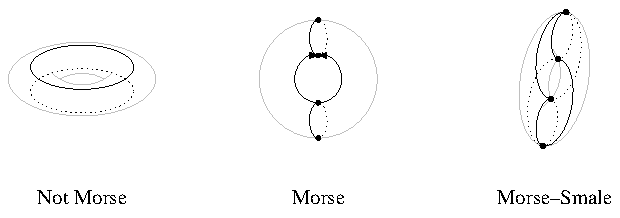
\includegraphics[width=0.82\textwidth]{figures/Fig_059_PDF138_Book126.pdf}
  \caption{高度函数分别不是 Morse 函数、是 Morse 函数及是 Morse--Smale 函数（原书 p.126）}
  \label{fig:morse-torus}
\end{figure}
\end{example}


现在设 $f$ 是 Morse--Smale 函数。若两个临界点 $p,q$ 的指数相差 $1$，则它们之间只有有限条流轨迹，因为此时 $\dim\operatorname{Desc}(p)\cap\operatorname{Asc}(q)=1$。可以按如下方式给每条轨迹赋予符号。先为所有 $\operatorname{Desc}(p)$ 选定定向；再要求分解
\[
  T_pM=T_p\operatorname{Desc}(p)\oplus T_p\operatorname{Asc}(p)
\]
保持定向，这便自动确定了 $\operatorname{Asc}(p)$ 的定向。类似地，可以为 $\operatorname{Desc}(p)\cap\operatorname{Asc}(q)$ 定向，方法是要求存在 $T_xM$ 的正向基 $b_1,\ldots,b_n$，使前一部分向量给出 $T_x\operatorname{Desc}(p)$ 的正向基，后一部分向量给出 $T_x\operatorname{Asc}(q)$ 的正向基，而重叠部分给出交空间 $T_x\operatorname{Desc}(p)\cap\operatorname{Asc}(q)$ 的正向基。

\begin{definition}{Morse 复形}{morse-complex}
紧致可定向 Riemann 流形 $(M,g)$ 上 Morse--Smale 函数 $f$ 的 Morse 复形\index{morsefuxing@Morse 复形|hyperpage} $C_M^\bullet(M,g,f)$，是由临界点张成、按 Morse 指数分次的向量空间。具体地，
\[
  C_M^i(M,g,f)=k\operatorname{Crit}_i(f),\qquad
  dp=\sum_{\substack{\gamma:p\to q\\|q|=|p|+1}}(-1)^\gamma q.
\]
这里 $(-1)^\gamma$ 在 $\gamma$ 沿 $\operatorname{Desc}(p)\cap\operatorname{Asc}(q)$ 的正向时取 $+1$。
\end{definition}

\begin{theorem}{Morse 复形计算流形上同调}{morse-cohomology}
Morse 复形是一个上链复形，并且它的上同调就是流形 $M$ 的上同调。
\end{theorem}
\begin{proof}[证明梗概]
微分的次数显然为 $1$，而且平方为零。展开 $d^2$ 可得
\[
  d^2(p)=\sum_{\substack{\gamma_1:p\to q\\|q|=|p|+1}}
  \sum_{\substack{\gamma_2:q\to r\\|r|=|q|+1}}
  (-1)^{\gamma_1}(-1)^{\gamma_2}r;
\]
因此，微分的平方统计了经由一个中间临界点到达 $r$ 的所有方式。

因为 $p$ 与 $r$ 的指数相差 $2$，$\operatorname{Desc}(p)$ 与 $\operatorname{Asc}(r)$ 的交是二维的。这意味着从 $p$ 到 $r$ 的轨迹组成单参数族；在这些单参数族的边界处，轨迹会断裂成两段。反过来，若有两条次数为 $1$ 的轨迹，局部上就可以把它们变形为一条次数为 $2$ 的轨迹。每个断裂为两段的轨迹族都有两个端点，因而总有两个符号相反的贡献，在 $d^2$ 中彼此抵消。下图示意这种边界配对：
\begin{figure}[H]\centering
  \centering
  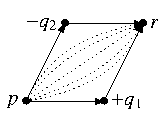
\includegraphics[width=0.32\textwidth]{figures/Fig_060_PDF139_Book127.pdf}
  \caption{一参数轨迹族的两种断裂端点（原书 p.127）}
  \label{fig:morse-broken-trajectories}
\end{figure}

为了证明 Morse 复形的上同调等于 $M$ 的上同调，把每个指数为 $i$ 的临界点与其上升流形对应起来。所有上升流形都是可缩的，并覆盖 $M$，因此给出一个胞腔分解；由此可以像定义单纯上同调那样定义胞腔上同调\bookcite[第 3 章]{111}。这个复形与 Morse 复形同构\bookcite[第 7.4 节]{28}。证明还有许多其他方法：使用同调而非上同调的论证见\bookcite[第 3 章]{123}；Witten\bookcite{256}则给出了完全不同的方法，把 Morse 复形与德拉姆复形联系起来。
\end{proof}

\begin{example}[驼峰球面的 Morse 复形]
考察一只竖立的、带有多个驼峰的球面。鞍点到两个驼峰各有一条路径，极小点到鞍点也有两条路径；后两条路径符号相反，因而彼此抵消。其 Morse 复形中，微分由鞍点映到两个极大点，而从极小点出发的两个贡献之和为 $1-1=0$。
若记极小点为 $p$、鞍点为 $q$，两个极大点为 $r_1,r_2$，则对应部分的微分为 $dp=(1-1)q=0$、$dq=r_1+r_2$。
\begin{figure}[H]\centering
  \centering
  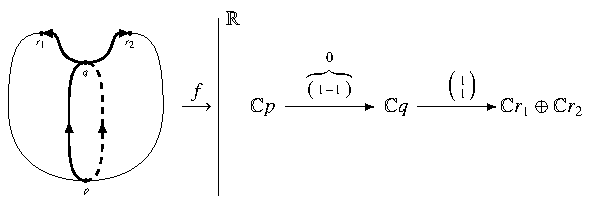
\includegraphics[width=0.72\textwidth]{figures/Fig_061_PDF140_Book128.pdf}
  \caption{驼峰球面上的临界点与 Morse 复形（原书 p.128）}
  \label{fig:morse-camel-sphere}
\end{figure}
\end{example}

\begin{note}\label{note:morse-homology-observation}
\textbf{观察 6.9.} 通过考察流形上函数的临界点所构成的复形，可以恢复流形的上同调；该复形的微分统计流轨迹。
\end{note}

\subsection{Morse 理论的动力学观点}\label{subsec:morse-dynamics}
现在用辛几何重新表述 Morse 理论。关于辛几何的背景，可参阅\bookcite{52,182}。回忆一下，辛流形是一个 $2n$ 维光滑实流形 $X$，带有闭且非退化的 $2$-形式 $\omega$：
\[
  d\omega=0,\qquad \omega(X,-)=0\Longrightarrow X=0.
\]
给定光滑函数 $h$，定义向量场 $X_h$ 使得
\[
  dh=\omega(-,X_h)=-\iota_{X_h}\omega,
\]
并定义流 $\phi_t^h\colon X\to X$，满足
\[
  \frac{d}{dt}\phi_t^h(x)=X_h(\phi_t^h(x)).
\]
函数 $h$ 通常称为 Hamilton 函数，该流称为 Hamilton 流\index{hamiltonliu@Hamilton 流|hyperpage}。Hamilton 流保持辛形式和 Hamilton 函数不变：
\[
  \frac{d}{dt}(\phi_t^h)^*\omega
  =\mathcal L_{X_h}\omega
  =\iota_{X_h}d\omega+d\iota_{X_h}\omega=0-d^2h=0,
\]
\[
  \frac{d}{dt}(\phi_t^h)^*h
  =\mathcal L_{X_h}h=dh(X_h)=\omega(X_h,X_h)=0.
\]
从物理角度看，Hamilton 函数表示系统总能量，而它在流下不变就意味着能量守恒。

辛流形的标准例子是流形 $M$ 的余切空间 $T^*M$，其上带有 $2$-形式
\[
  \omega=\sum_i dp_i\wedge dq_i,
\]
其中 $q_i$ 是 $M$ 上的局部坐标，$p_i$ 是余切空间中相对于基 $\{dq_i\}$ 的坐标。$q_i$ 称为位置坐标，$p_i$ 称为动量坐标。在这些坐标下，向量场 $X_h$ 的形式为
\[
  X_h=\sum_i\frac{\partial h}{\partial p_i}\frac{\partial}{\partial q_i}
       -\sum_i\frac{\partial h}{\partial q_i}\frac{\partial}{\partial p_i}.
\]

若 $f$ 是 Riemann 流形 $(M,g)$ 上的函数，可以沿投影映射将它拉回到 $T^*M$ 上。对应的 Hamilton 向量场为
\[
  X_f=-\sum_i\frac{\partial f}{\partial q_i}\frac{\partial}{\partial p_i}.
\]
% [Tutor Note: 符号约定需自行统一。原文 p.128 定义 $dh=\iota_{X_h}\omega$，但 p.129 的 $X_h=\sum_i\frac{\partial h}{\partial p_i}\frac{\partial}{\partial q_i}-\sum_i\frac{\partial h}{\partial q_i}\frac{\partial}{\partial p_i}$ 与 $\omega=\sum_i dp_i\wedge dq_i$ 差一负号；按已给的 $X_h$ 反推应为 $dh=\omega(-,X_h)=-\iota_{X_h}\omega$。后文例 6.56（原书 p.156）用 $\dot q_i=-\partial H/\partial p_i$、$\dot p_i=\partial H/\partial q_i$，即后一约定；推导 Floer 条带的 Cauchy--Riemann 方程时必须始终沿用同一约定。]
从物理角度看，这个动力系统颇为奇怪：粒子的动量会变化，但位置不变。这是因为 $f$ 含有势能项（依赖坐标 $q_i$），却不含动能项（依赖坐标 $p_i$）。流 $\phi_t^f$ 把底空间 $M\subset T^*M$ 移到另一个 $n$ 维子流形 $\phi_t^fM\subset T^*M$。$f$ 的临界点恰好是 $\phi_t^fM$ 与 $M$ 的交点，因为在这些点上流是静止的，即 $X_f(x)=0$。

若沿一条连接两个临界点的 Morse 轨迹 $\gamma$ 作流，它会扫出一个边界落在 $M\cup\phi_t^fM$ 上的曲面。这个曲面有一个特殊性质：它是全纯圆盘。为了说明这一点，先在 $T^*M$ 上定义复结构。切丛 $TM$ 有自然的复流形结构：若 $q_i$ 是 $M$ 上的局部坐标，则 $TM$ 上相对于局部基 $\frac{\partial}{\partial q_i}$ 的坐标为 $q_i,\dot q_i$；组合为
\[
  z_i=q_i+i\dot q_i
\]
便得到 $TM$ 上的全纯坐标。若 $M$ 带有度量 $g$，则切丛与余切丛之间有微分同胚
\[
  \phi_g\colon TM\to T^*M,\qquad X\longmapsto g(X,-).
\]
在该微分同胚下，坐标 $p_i$ 对应于 $g_{ij}\dot q_j$。这里使用 Einstein 求和约定，并记 $g_{ij}=g(\frac{\partial}{\partial q_i},\frac{\partial}{\partial q_j})$。

\begin{lemma}{Morse 轨迹给出全纯映射}{morse-trajectory-holomorphic}
映射
\[
  \psi\colon\mathbb R+[0,\epsilon]i\to T^*M,
  \qquad s+ti\longmapsto\phi_{t}^{h}\gamma(s)
\]
是全纯的。
\end{lemma}
\begin{proof}[证明梗概]
只需验证 Cauchy--Riemann 方程。沿 $s$ 方向的导数为 $(\nabla f,0)$，因为 $q_i$ 坐标沿 Morse 流变化，而 $p_i$ 不变。沿 $t$ 方向的导数只改变 $p_i$ 坐标，所以为 $\bigl(0,-\frac{\partial f}{\partial q_i}\bigr)$。改用 $(q_i,\dot q_i)$ 坐标后，得到
\[
  \frac{\partial\psi}{\partial s}=(\nabla f,0),\qquad
  \frac{\partial\psi}{\partial t}=(0,-\nabla f)
  =-i\frac{\partial\psi}{\partial s},
\]
这正是所需的 Cauchy--Riemann 方程。
\end{proof}

我们可以将条带 $\mathbb R+[0,\epsilon]i$ 全纯地识别为去掉 $\{1,-1\}$ 两点的单位圆盘 $D=\{z\in\mathbb C\mid|z|\le1\}$。于是 $\psi$ 可看成全纯映射
\[
  \psi\colon D\setminus\{-1,1\}\to T^*M,
\]
且当 $u\in[0,\frac12]$ 时 $\psi(e^{2\pi iu})\in M$，当 $u\in[\frac12,1]$ 时 $\psi(e^{2\pi iu})\in\phi_\epsilon^hM$。我们称这样的映射为全纯二边形（或双边形）。
\begin{figure}[H]\centering
  \centering
  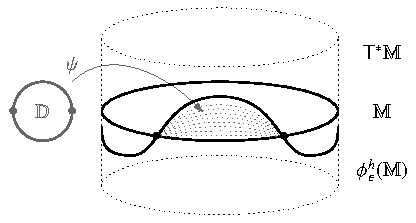
\includegraphics[width=0.62\textwidth]{figures/Fig_062_PDF142_Book130.pdf}\quad
  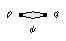
\includegraphics[width=0.22\textwidth]{figures/Fig_063_PDF142_Book130.pdf}
  \caption{Morse 流条带与余切丛中的全纯二边形（原书 p.130）}
  \label{fig:morse-holomorphic-bigon}
\end{figure}

从这个新观点看，Morse 上链复形由 $L:=\phi_\epsilon^hM$ 与 $M$ 的交点张成，而微分统计全纯二边形：
\[
  C_M^\bullet(M,g,f)=CF^\bullet(L,M)
  :=\bigoplus_{p\in L\cap M}kp,
  \qquad dp=\sum_{\substack{q\in L\cap M\\|q|=|p|+1}}
             \sum_{\psi:p\to q}\pm q.
\]

在这一新形式体系中，Morse 指数该如何解释？首先，若 $M$ 可定向，则可以给它配上体积形式
\[
  \Omega_{\mathbb R}=\sqrt{\det g_{ij}}\,dq_1\wedge\cdots\wedge dq_n.
\]
这个体积形式可在 $TM$ 上传递为复体积形式
\[
  \Omega_{\mathbb C}=\sqrt{\det g_{ij}}\,dz_1\wedge\cdots\wedge dz_n.
\]
考察它在 $T_pL$ 上的限制，像落在 $\mathbb C$ 中的一条直线 $\mathbb Re^{i\theta_p}$ 上，其中 $\theta_p\in\mathbb R/\pi\mathbb Z$。在此情形中，实际上可以把它提升为函数 $\theta_L\colon L\to\mathbb R$，这个提升函数称为分次。注意，$M$ 本身带有分次 $\theta_M\colon M\to\mathbb R$，其定义为 $p\mapsto0$，因为 $\Omega_{\mathbb C}|_{T_pM}$ 为实值。

若 $p$ 是 $L$ 与 $M$ 的交点，则存在酉变换 $U\colon T_p(T^*M)\to T_p(T^*M)$，把 $T_pL$ 映到 $T_pM$。取 $\Delta\in[0,\pi)$ 使 $\det U=\pm e^{i\Delta}$。交点 $p$ 的次数定义为
\[
  \deg p=\frac{\Delta-(\theta_M-\theta_L)}{\pi}.
\]
由于 $U^*(\Omega|_{T_pM})=\det(U)\,\Omega|_{T_pL}$，相位差 $\theta_M-\theta_L$ 必属于 $\Delta+\pi\mathbb Z$，所以 $\deg p$ 是整数。

\begin{example}[圆上的 Morse 函数与交点次数]
令 $M=\mathbb R/2\pi\mathbb Z$，取标准度量，并令 Hamilton 函数 $h=\cos q$。它在 $q=0,\pi$ 处有两个临界点 $p_0,p_1$。辛流形 $T^*M$ 是一个圆柱；除 $q=0,\pi$ 两处的静止轨迹外，其余轨迹都是竖直直线。
\begin{figure}[H]\centering
  \centering
  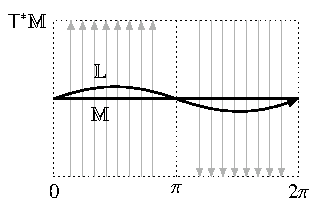
\includegraphics[width=0.78\textwidth]{figures/Fig_064_PDF143_Book131.pdf}
  \caption{圆的余切丛及 Hamilton 变形后的交点（原书 p.131）}
  \label{fig:circle-cotangent-flow}
\end{figure}
图中有两个拉格朗日子流形 $M$ 与其流动后的像 $L=\phi_\epsilon^h(M)$。$\theta_L$ 可取为 $T_pL$ 在每点处的相位，因此 $\theta_{p_0}=\epsilon$、$\theta_{p_1}=-\epsilon$。把 $T_pL$ 映到 $T_pM$ 的酉矩阵为
\[
  U_0=e^{i(\pi-\epsilon)},\qquad U_1=e^{i\epsilon},
\]
于是
\[
  \deg p_0=\frac{\pi-\epsilon-(0-\epsilon)}{\pi}=1,
  \qquad
  \deg p_1=\frac{\epsilon-(0+\epsilon)}{\pi}=0.
\]
\end{example}

\begin{note}\label{note:morse-intersections-observation}
\textbf{观察 6.12.} 通过考察余切丛中的零截面 $M\subset T^*M$ 与其 Hamilton 变形的交点，可以恢复流形的上同调；微分统计交点之间的全纯条带。
\end{note}

\subsection{环路空间的同调}\label{subsec:loop-space-homology}
现在考察动力学谱系的另一端，即 Hamilton 函数只有动能项的情形：
\[
  h=\frac12g^{ij}p_ip_j.
\]
这描述粒子在 $M$ 上自由运动。经典力学告诉我们，这种粒子以恒定速度沿 $M$ 上的测地线运动。在 $T^*M$ 的零截面 $M$ 上，$p_i=0$，所以速度为零，什么也不会发生：$\phi_\epsilon^h(M)=M$。

取余切丛的一条纤维 $L=T_x^*M$，并利用度量把它与 $T_xM$ 识别。点 $(q_i,\dot q_i)$ 在 $\phi_t^h$ 下的像，会沿 $\dot q_i$ 方向的测地线移动，距离为 $t\|\dot q_i\|$。

因此，$\phi_\epsilon^h(L)$ 与 $L$ 的交点表示从 $x$ 出发又回到 $x$ 的闭测地线。若 $\gamma\colon[0,1]\to M$ 是长度为 $\ell$ 的一条简单闭测地线，那么对任意 $z\in\mathbb Z$，点
\[
  \left(x,\frac{z\ell\,\dot\gamma(0)}{\epsilon\|\dot\gamma(0)\|}\right)
\]
都属于 $\phi_\epsilon^h(L)\cap L$；所有交点都由此方式得到。

考察以 $x$ 为基点的 $M$ 上所有环路组成的空间
\[
  \mathcal L_x(M)=\{\gamma\colon S^1\to M\mid\gamma(0)=x\}.
\]
环路空间上有函数 $f\colon\mathcal L_x(M)\to\mathbb R$，把每条环路映到其长度
\[
  f(\gamma)=\int_{S^1}\|\dot\gamma(t)\|\,dt.
\]
测地环路正是该函数的临界点，因此可以构造一个类似 Morse 复形的对象来计算 $\mathcal L_x(M)$ 的同调。它仍应由 $L$ 与 $\phi_t^h(L)$ 的交点张成。但此时交点不再来自静止轨迹，而来自周期轨迹。每个交点 $u$ 都对应一条从 $u$ 出发又回到 $u$ 的流线 $\widetilde\upsilon\colon[0,\epsilon]\to T^*M$。因此，微分应统计具有如下极限条件的条带：
\[
  \psi\colon\mathbb R+[0,\epsilon]i\to T^*M,
  \qquad s+ti\longmapsto\phi_t^h\gamma(s),
\]
其中 $s\to\pm\infty$ 时的极限恰好是上述流线。与 Morse 情形一样，这些条带应满足适当版本的 Cauchy--Riemann 方程。要使这一构造成立并不容易，因为无限维空间上的 Morse 理论技术性很强。

\begin{example}[圆周的环路空间]
令 $M=S^1$，则 $T^*M$ 是圆柱。标准坐标为 $(q,p)$，其中 $q$ 表示圆上的角度，$p$ 表示圆柱的高度。原点处的竖直线为 $L=T_0S^1$，而 $\phi_t^h(L)$ 是绕圆柱盘绕的螺线，其方程为 $q=tp$。交点为
\[
  (0,2\pi k/t),\qquad k\in\mathbb Z.
\]
环路空间按绕数分成连通分支，每个分支恰有一个临界点，所以不同临界点之间没有轨迹。因此，由 $\phi_t^h(L)$ 与 $L$ 的交点张成的复形，其微分为零。
\end{example}

\begin{note}\label{note:loop-space-intersections}
\textbf{观察 6.14.} 通过考察余切纤维 $T_x^*M$ 与其 Hamilton 变形的交点，可以计算流形环路空间的同调；微分统计交点之间的全纯条带。
\end{note}

\section{基本 Fukaya 范畴}\label{sec:basic-fukaya}
上面的讨论打开了若干推广方向。我们可以在任意辛流形中的拉格朗日子流形\index{lagelangriziliuxing@拉格朗日子流形|hyperpage}之间发展交理论，并通过考察全纯 $n$ 边形，把微分提升为高阶乘积。这就引出 Fukaya 范畴的思想。不过，Fukaya 范畴有许多不同概念，具体取决于辛流形的类型和要纳入的拉格朗日子流形种类。本节将定义最基本的版本，并详细讨论最简单的例子。

\takeaway{在带柱状端的 Liouville 流形中，正合紧致拉格朗日子流形之间的 Floer 复形由横截交点张成，高阶积通过计数满足边界条件的伪全纯多边形定义；正合性使求和有限并排除起泡，由此得到 $\mathbb Z_2$-分次的 $A_\infty$ 预范畴，存在复体积形式时可提升为 $\mathbb Z$-分次。}

\subsection{设定}\label{subsec:fukaya-setting}
为了得到合理的理论，当然需要限制辛流形与拉格朗日子流形的几何复杂度。因此，我们从一个与余切丛情形较为接近的设定开始。

\begin{definition}{Liouville 流形与 Liouville 域}{liouville-manifold}
若存在 $1$-形式 $\theta$ 使得 $\omega=d\theta$，则称辛流形 $(X,\omega)$ 为正合辛流形\index{zhenghexinliuxing@正合辛流形|hyperpage}。$1$-形式 $\theta$ 称为 Liouville 形式\index{liouvillexingshi@Liouville 形式|hyperpage}；满足 $\omega(X_\theta,-)=\theta$ 的向量场 $X_\theta$ 称为 Liouville 向量场\index{liouvillexiangliangchang@Liouville 向量场|hyperpage}。

若存在带边界的紧致流形 $X_0$ 满足以下条件，则称 $(X,\theta)$ 为具有柱状端的 Liouville 流形：
\begin{itemize}
  \item $X$ 由在 $X_0$ 的边界上接出柱体得到：
  \[
    X=X_0\cup_{\partial X_0}(\partial X_0\times[1,+\infty));
  \]
  \item 在柱体上，$X_\theta$ 指向外侧：
  \[
    X_\theta\big|_{\partial X_0\times[1,+\infty)}
    =r\frac{\partial}{\partial r},
  \]
  其中 $r$ 是 $(1,+\infty)$ 上的坐标。
\end{itemize}
紧致流形 $X_0$ 称为 Liouville 域\index{liouvilleyu@Liouville 域|hyperpage}\bookcite{15}。
\end{definition}

\begin{example}[余切丛上的 Liouville 结构]
带柱状端的 Liouville 流形\index{daizhuzhuangduandeliouvilleliuxing@带柱状端的 Liouville 流形|hyperpage}的标准例子是紧致流形 $M$ 的余切丛 $X=T^*M$。其 Liouville 形式为 $\theta=p_i\,dq_i$，相应的 Liouville 向量场为 $X_\theta=p_i\frac{\partial}{\partial p_i}$。$X_0$ 可取余切丛的单位球盘 $X_0=\{x\in X\mid\|p\|\le1\}$，坐标 $r$ 可取为 $\|p\|$（定义 $p$ 的范数时需要在 $M$ 上选取度量）。
\end{example}

\begin{definition}{正合拉格朗日子流形}{exact-lagrangian}\index{zhenghelagelangriziliuxing@正合拉格朗日子流形|hyperpage}
拉格朗日子流形是一个定向的 $n$ 维子流形 $L$，满足 $\omega(TL,-)=0$。若存在函数 $f\colon L\to\mathbb R$ 使得 $\theta|_L=df$，则称 $L$ 为正合的；若在柱体 $\partial X_0\times[1,+\infty)$ 上 Liouville 向量场 $X_\theta$ 与 $L$ 相切，则称 $L$ 具有锥形端\index{zhuixingduan@锥形端|hyperpage}。

若对每个交点 $p\in L_1\cap L_2$ 都有 $T_pX=T_pL_1\oplus T_pL_2$，则称两个拉格朗日子流形 $L_1,L_2$ 横截相交\index{hengjiexiangjiao@横截相交|hyperpage}。
\end{definition}

\begin{example}[余切丛中的零截面与纤维]
余切丛的底空间是紧致的正合拉格朗日子流形，而任意点 $x\in M$ 处的余切纤维是具有锥形端的正合拉格朗日子流形。两种情形下 $\theta$ 的限制都是零，因而是常值函数的微分。底空间与余切纤维在 $x$ 处横截相交。
\end{example}

\begin{definition}{相容的几乎复结构}{almost-kaehler}
给定 $2n$ 维辛流形 $(X,\omega)$，几乎复结构\index{jinfujiegou@几乎复结构|hyperpage}\index{fujiegou@复结构|hyperpage}是一个映射 $J\colon TX\to TX$，满足 $J^2=-1$。若
\[
  g(-,-):=\omega(-,J-)
\]
是 $X$ 上的 Riemann 度量，就称 $J$ 与 $\omega$ 相容。三元组 $(X,\omega,J)$ 称为几乎 Kähler 流形\index{khlerliuxing@Kähler 流形|hyperpage}。
\end{definition}

\begin{note}\label{note:almost-complex-structure}
\textbf{注 6.20.} 若 $X$ 是复流形（即存在坐标图 $\phi_U\colon U\to\mathbb C^n$，使得 $\phi_U\circ\phi_{U'}^{-1}$ 为全纯映射），就可以把 $X$ 看作实流形，并把映射 $J\colon TX\to TX:z\mapsto iz$ 看作几乎复结构。反过来通常不成立：并非每个几乎复结构都来自复坐标图册。若确实如此，就可以从定义中去掉“几乎”二字，称之为复结构，此时流形称为 Kähler 流形。
\end{note}

\begin{note}\label{note:compatible-almost-complex-contractible}
\textbf{注 6.21.} 对给定的 $(X,\omega)$，与 $\omega$ 相容的几乎复结构所成空间是可缩的。对所有复结构所成的空间，这一结论则不成立。
\end{note}

\begin{definition}{伪全纯映射}{pseudoholomorphic-map}
对任意开集 $U\subset\mathbb C$，若映射 $\phi\colon U\to X$ 满足 Cauchy--Riemann 方程
\[
  \frac{\partial\phi(u+iv)}{\partial u}
  +J\frac{\partial\phi(u+iv)}{\partial v}=0,
\]
则称 $\phi$ 为伪全纯映射\index{weiquanchunyingshe@伪全纯映射|hyperpage}。
\end{definition}

\begin{example}[复代数环面的 Liouville 结构]
\par
复代数环面 $(\mathbb C^*)^n$ 可通过 $z_i=e^{p_i+iq_i}$ 与 Liouville 流形 $(T^*(S^1)^n,p_i\,dq_i)$ 识别；这给出 $X=T^*(S^1)^n$ 上的复结构。因此 $(X,\omega,J)$ 是 Kähler 流形，并且
\[
  \omega=d\theta=\sum_i dp_i\wedge dq_i
  =\frac{i}{2}\sum_i d\ln z_i\wedge d\ln\bar z_i
  =\frac{i}{2}\sum_i\frac{dz_i}{z_i}\wedge\frac{d\bar z_i}{\bar z_i},
\]
\[
  J=\sum_i\left(i\frac{\partial}{\partial z_i}\otimes dz_i
   -i\frac{\partial}{\partial\bar z_i}\otimes d\bar z_i\right)
  =\sum_i\left(\frac{\partial}{\partial q_i}\otimes dp_i
   -\frac{\partial}{\partial p_i}\otimes dq_i\right),
  \qquad
  g=\sum_i(dp_i\otimes dp_i+dq_i\otimes dq_i).
\]
若 $f\in\mathbb C[X_1^{\pm1},\ldots,X_n^{\pm1}]$，且
\[
  X_f:=\{(z_1,\ldots,z_n)\in(\mathbb C^*)^n\mid f(z_1,\ldots,z_n)=0\}
\]
是光滑子流形，那么 $(X_f,\theta|_{X_f})$ 是带柱状端、具有相容复结构的 Liouville 流形。
\end{example}

\subsection{初步尝试定义 Fukaya 范畴}\label{subsec:fukaya-first-definition}
本节中，$(X,\theta)$ 表示带柱状端的 Liouville 流形。记 $\omega=d\theta$ 为其辛形式，并假设它带有一个相容的几乎复结构 $J$ 及其诱导度量 $g$。

\begin{definition}{Floer 复形与全纯多边形乘积}{floer-complex}
给定两个横截相交的紧致正合拉格朗日子流形 $L_1,L_2\subset X$，Floer 复形定义为 $\mathbb Z_2$-分次向量空间
\[
  CF_k^{\pm}(L_1,L_2):=\bigoplus_{p\in L_1\cap L_2}kp.
\]
交点 $p$ 的次数按如下方式确定。取 $T_pL_1$ 与 $T_pL_2$ 的正向基 $v_1,\ldots,v_n$ 和 $w_1,\ldots,w_n$。若 $v_1,\ldots,v_n,w_1,\ldots,w_n$ 构成 $T_pX$ 的正向基，则令 $\deg p=0$；若它构成负向基，则令 $\deg p=1$。
设 $L_0,\ldots,L_k$ 是两两横截相交的紧致正合定向拉格朗日子流形，则定义
\[
  \mu\colon CF_k^{\pm}(L_1,L_0)\otimes\cdots\otimes
    CF_k^{\pm}(L_k,L_{k-1})\to CF_k^{\pm}(L_k,L_0)
\]
为
\[
  \mu(p_1,\ldots,p_k):=\sum_{p_0\in L_0\cap L_k}\sum_{\psi}
     \sigma_\psi\,p_0.\tag{6.1}\label{eq:fukaya-product}
\]
这里对所有满足下列条件的伪全纯映射
\[
  \psi\colon D\setminus\{e^{2r\pi i/(k+1)}\mid r\in\mathbb Z\}\to X
\]
求和：
\begin{itemize}
  \item 边界映到拉格朗日子流形上：若 $t\in(i,i+1)$，则 $\psi(e^{2\pi it/(k+1)})\in L_i$；
  \item 在单位根 $\zeta_r=e^{2r\pi i/(k+1)}$ 处的极限对应交点，即 $\lim_{t\to\zeta_r}\psi(z)=p_r$；
  \item 映射按固定各 $\zeta_r$ 的圆盘重参数化取等价类；
  \item 映射不能再作形变；
  \item 每一项都带有符号 $\sigma_\psi$，该符号取决于拉格朗日子流形的定向，也可能取决于其他附加数据。
\end{itemize}
图示如下；每个交点处的小箭头表示相应态射的方向：
\begin{figure}[H]\centering
  \centering
  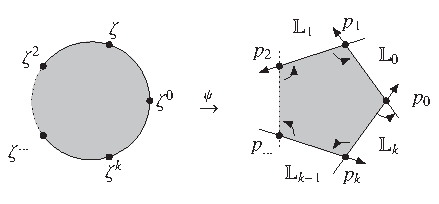
\includegraphics[width=0.66\textwidth]{figures/Fig_065_PDF148_Book136.pdf}
  \caption{由全纯多边形定义高阶乘积（原书 p.136）}
  \label{fig:fukaya-holomorphic-polygons}
\end{figure}
\end{definition}

从图像上看，这类映射可画成边界依次落在各拉格朗日子流形上的圆盘，并在各角点处标出态射方向。目标空间的角点刻意画成非光滑的形状，以强调 $\psi$ 在 $\zeta_i$ 处不必全纯。若拉格朗日子流形是一维的，那么对每个次数为奇数且 $i>0$ 的 $p_i$，当其目标拉格朗日子流形的正向与圆盘边界的正向相反时，$\sigma_\psi$ 会多出一个 $-1$ 因子。

我们希望这些乘积定义良好并满足 $A_\infty$ 关系；但要做到这一点，还必须处理若干技术问题。

\subsection{模空间}\label{subsec:fukaya-moduli-spaces}
首先要精确说明“映射不能再作形变”是什么意思。给定交点序列 $p_0,\ldots,p_k$，可以构造模空间 $\mathcal M(p_0,\ldots,p_k)$，其元素是满足相应边界条件的映射，按重参数化取等价类。模空间自然按 $\psi$ 相对于边界 $\bigcup_iL_i$ 的同调类分解为不交并：
\[
  \mathcal M(p_0,\ldots,p_k)=
  \coprod_{u\in H_2(X,\cup_iL_i)}\mathcal M_u.
\]
理想情况下，每个 $\mathcal M_u$ 都应当是维数等于预期维数的光滑可定向流形；然而，这并不容易做到。
\begin{itemize}
  \item 为保证光滑性，必须假设 $J$ 是通有的；甚至可能要通过加入依赖时间的 Hamilton 流和几乎复结构来扰动 Cauchy--Riemann 方程。这类似于构造 Morse 复形时要求函数为 Morse--Smale 函数。
  \item 为保证可定向性，拉格朗日子流形需要可定向，并带有自旋结构\bookcite[II.11]{218}。若 $L$ 是闭曲线，它有两种自旋结构：平凡自旋结构与非平凡自旋结构，分别对应圆上的两种局部 $\mathbb Z_2$-系。非平凡自旋结构可通过在曲线上选取一个标记点来描述，在该点处平凡化失效。圆盘边界上的每个标记点都会在 $\sigma_\psi$ 中额外引入一个负号。
\end{itemize}

下文中我们假设 $\mathcal M_u$ 是可定向流形。当 $\dim\mathcal M_u=0$ 时，它是由离散点 $\psi$ 组成的集合，每个点带有表示定向的符号 $\sigma_\psi$。我们只对零维 $\mathcal M_u$ 中的映射求和。

为了保证上述定义良好，参与求和的映射 $\psi$ 总数必须有限。这一点并不显然：即使每个零维 $\mathcal M_u$ 都只含有限多个点，它们的总数仍可能无限。幸运的是，我们施加的限制可以帮助解决这个问题。

\begin{lemma}{正合性保证 Floer 乘积有限}{exactness-finite-floer-sum}
若辛流形及所有紧致拉格朗日子流形都是正合的，则式~\eqref{eq:fukaya-product} 中的和是有限和。
\end{lemma}
\begin{proof}[证明梗概]
这要用到 Gromov 紧致性定理\bookcite{100}：给定面积上界后，面积小于该上界的全纯映射只有有限多个。由于 $\omega$ 正合，映射 $\psi$ 的面积可表示为边界上的积分，再拆成各拉格朗日子流形上的积分之和：
\[
  \int_D\psi^*\omega=\int_Dd\psi^*\theta
  =\int_{\partial D}\psi^*\theta
  =\sum_i\int_{p_i}^{p_{i+1}}\theta|_{L_i}.
\]
由正合性，每一项都可写成
\[
  \int_{p_i}^{p_{i+1}}\theta|_{L_i}
  =\int_{p_i}^{p_{i+1}}df_i=f_i(p_{i+1})-f_i(p_i),
\]
其中 $f_i\colon L_i\to\mathbb R$ 是 $\theta|_{L_i}$ 的原函数。因为 $L_i$ 紧致，积分被 $f_i$ 的最大值与最小值之差控制，因此 $\psi$ 的面积有界。
\end{proof}

\subsection{泡}
为了确保这些乘积满足 $A_\infty$ 关系，我们希望仿照定理~\ref{thm:morse-cohomology} 中 Morse 微分的情形。在那里，我们把两条轨迹粘在一起，再将它们变形为一个单参数族；这个轨迹族的断裂端点对应另外一对轨迹，而这两端的贡献在 $d^2$ 中相消。

这里也可以做类似的事：把两个圆盘沿一个共同标记点粘合起来，对粘合结果作形变，再使它断裂为另外两个圆盘。形变族的两个端点分别对应 $A_\infty$ 关系中的项，例如 $\mu_1(\mu_4(p_1,\ldots,p_4))$ 和 $\mu_3(p_1,\mu_2(p_2,p_3),p_4)$；它们符号相反，因而相消。

至少理论上应当如此；但实际上还会出现两类退化，它们并不对应 $A_\infty$ 公理中的项。这种现象称为起泡\index{qipao@起泡|hyperpage}：
\begin{itemize}
  \item \textbf{圆盘泡}\index{yuanpanpao@圆盘泡|hyperpage}发生在额外圆盘从某段边界冒出时。该圆盘可看作零元乘积 $\mu_0$ 的额外贡献；此时得到的不是普通 $A_\infty$ 结构，而是带曲率的 $A_\infty$ 结构。
  \item \textbf{球面泡}\index{qiumianpao@球面泡|hyperpage}发生在球面从圆盘内部切离时。
\end{itemize}
泡类似于含有环路的 Morse 轨迹。在 Morse 理论中，由于轨迹沿 Morse 函数单调上升，这种情形不可能发生。正合情形下也可以得到类似结论。
\begin{figure}[H]\centering
  \centering
  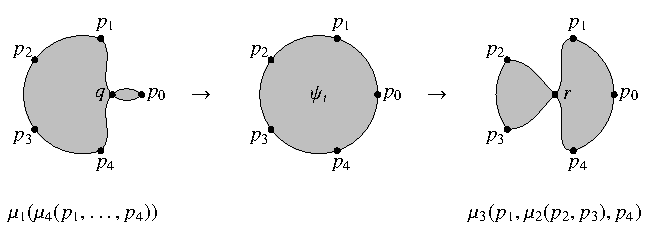
\includegraphics[width=0.78\textwidth]{figures/Fig_066_PDF150_Book138.pdf}
  \caption{模空间边界上的断裂圆盘（原书 p.138）}
  \label{fig:fukaya-moduli-boundary}
\end{figure}
\begin{figure}[H]\centering
  \centering
  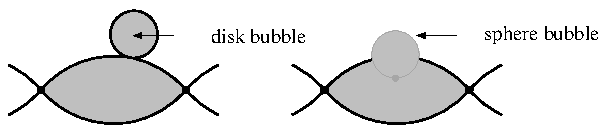
\includegraphics[width=0.58\textwidth]{figures/Fig_067_PDF150_Book138.pdf}
  \caption{圆盘泡与球面泡（原书 p.138）}
  \label{fig:fukaya-disk-sphere-bubbles}
\end{figure}

\begin{lemma}{$A_\infty$ 关系}{fukaya-ainfty-relations}
乘积 $\mu_k$ 满足 $A_\infty$ 公理。
\end{lemma}
\begin{proof}[证明梗概]
在正合情形下，两类泡都会给出面积为零的映射 $\psi$。利用这些映射可以构造出无穷多个面积受某个常数控制的映射，这与 Gromov 紧致性定理矛盾。

完整证明见 Seidel\bookcite[第二部分]{218}。证明中要构造模空间 $\mathcal M_u(p_0,\ldots,p_k)$ 的紧化，其边界由含有较少标记点的模空间之积构成。在这些空间上，$A_\infty$ 乘积可解释为边界算子 $d$，于是 $A_\infty$ 关系便来自 $d^2=0$。
\end{proof}
% [Tutor Note: “$J$ 一般”只保证模空间在预期维数处光滑，这里省略了两处：一是标记点处的赋值映射也须横截，否则要用含时 Hamilton 扰动或虚拟基本类框架；二是正合性只排除面积为零的泡，还须先证明面积有正下界，才能由 Gromov 紧致性得到有限性。完整细节见 Seidel 书第二部分（文献 218）。]

\subsection{Floer 上同调}\label{subsec:floer-cohomology}
处理好上述问题后，便得到 Floer 理论的基本定理。

\begin{theorem}{Floer 上同调不变性}{floer-invariance}
（Floer\bookcite{79}）设 $k$ 是特征为 $2$ 的域，$(X,\theta,J)$ 是带柱状端的 Liouville 流形，并带有相容的几乎复结构。设 $L_1,L_2$ 是紧致、正合、定向的拉格朗日子流形，二者横截相交，并假设 $J$ 通有。
\begin{enumerate}[label=(\roman*)]
  \item $(CF_k^{\pm}(L_1,L_2),\mu_1)$ 是一个 $\mathbb Z_2$-分次复形。
  \item 若 $J_t$（$t\in[0,1]$）是一族几乎复结构，那么只要 $J_0,J_1$ 通有，就有拟同构
  \[
    CF_k^{\pm}(L_1,L_2)_{J_0}\simeq CF_k^{\pm}(L_1,L_2)_{J_1}.
  \]
  \item 若 $\phi_t^h$ 是 Hamilton 流，那么只要所涉及的拉格朗日子流形横截相交，就有拟同构
  \[
    CF_k^{\pm}(L_1,L_2)\simeq
    CF_k^{\pm}(\phi_\epsilon^hL_1,L_2)\simeq
    CF_k^{\pm}(L_1,\phi_\epsilon^hL_2).
  \]
\end{enumerate}
换言之，Floer 上同调是一个不变量，只依赖于拉格朗日子流形的 Hamilton 同痕类和辛结构。
\end{theorem}

\begin{note}\label{note:floer-spin-structure}
\textbf{注 6.29.} 如前所述，若要使该定理对特征不为 $2$ 的域成立，拉格朗日子流形必须配备自旋结构\bookcite[II.11]{218}。
\end{note}

\subsection{预范畴}\label{subsec:fukaya-precategories}
现在希望把这些数据打包成一个范畴。对象应是 $X$ 中正合、紧致的拉格朗日子流形，态射空间应为 Floer 复形。遗憾的是，事情没有这么简单：态射空间只在横截相交的拉格朗日子流形之间定义，因此对象与自身之间尤其没有态射空间。第三章第 3.4.4 节介绍的预范畴可以解决这个问题。

\begin{definition}{基本 Fukaya 预范畴}{basic-fukaya-precategory}
设 $(X,\theta,J)$ 是带柱状端的 Liouville 流形，并带有相容的几乎复结构。基本 Fukaya 预范畴 $\widehat{\mathrm{Fuk}}^{\pm}(X,\theta,J)$ 是具有下列数据的 $\mathbb Z_2$-分次预范畴：
\begin{itemize}
  \item 对象是 $X$ 中配有自旋结构的紧致、定向、正合拉格朗日子流形；
  \item 横截序列由满足以下条件的拉格朗日子流形元组组成：元组中各子流形两两横截相交、交点各不相同，且 $J$ 通有；
  \item 对每个 $(L_1,L_2)\in\widehat{\mathrm{Fuk}}^{\pm}(X,\theta,J)^2_{\mathrm{tr}}$，置
  \[
    \widehat{\mathrm{Fuk}}^{\pm}(L_1,L_2)=CF_k^{\pm}(L_1,L_2);
  \]
  \item 对每个 $(L_0,\ldots,L_k)\in\widehat{\mathrm{Fuk}}^{\pm}(X,\theta,J)^{k+1}_{\mathrm{tr}}$，定义前文给出的乘积 $\mu_k$。
\end{itemize}
\end{definition}

\begin{lemma}{基本 Fukaya 预范畴具有足够多拟同构}{fukaya-precategory-quasi-isomorphisms}
$\widehat{\mathrm{Fuk}}^{\pm}(X,\theta,J)$ 是一个具有足够多拟同构的预范畴。
\end{lemma}
\begin{proof}[证明梗概]
横截序列的任意子序列仍是横截的；又因为这里不会起泡，所以只要 $A_\infty$ 公理中的乘积有定义，这些公理就成立。

为证明它具有足够多拟同构，设 $L$ 是紧致拉格朗日子流形。由\bookcite[6.1]{252}可知，$L\subset X$ 的一个邻域与 $T^*L$ 同构。若在 $L$ 上选取一个 Morse--Smale 函数 $f$，并使每个连通分支上恰有一个局部极小值，就可以用该函数把 $L$ 流到 $\phi_\epsilon^fL$。这些极小值之和给出 $\widehat{\mathrm{Fuk}}^{\pm}(L,\phi_\epsilon^fL)$ 中的一个零次态射，它对应于
\[
  H^\bullet(L,k)\cong HCF_k^\bullet(L,\phi_\epsilon^fL)
\]
中的单位，因此是拟同构。

由于 $f$ 可以是 $L$ 上任意 Morse--Smale 函数，这样的拟同构有很多。给定其他一组拉格朗日子流形后，总能找到一个 $f$，使 $L_+=\phi_\epsilon^fL$ 与 $L_-=\phi_{-\epsilon}^fL$ 都和它们横截相交，并与 $J$ 相容。
\end{proof}

\begin{definition}{基本 Fukaya 范畴}{basic-fukaya-category}
基本 Fukaya 范畴 $\widehat{\mathrm{Fuk}}^{\pm}(X,\theta,J)$ 定义为相应基本 Fukaya 预范畴的范畴化。
\end{definition}

\begin{theorem}{基本 Fukaya 范畴与几乎复结构无关}{fukaya-complex-structure-invariance}
对两个不同的几乎复结构 $J_0,J_1$，Fukaya 范畴 $\widehat{\mathrm{Fuk}}^{\pm}(X,\theta,J_0)$ 与 $\widehat{\mathrm{Fuk}}^{\pm}(X,\theta,J_1)$ 之间存在 $A_\infty$ 拟同构。
\end{theorem}
\begin{proof}[证明梗概]
几乎复结构空间是可缩的，因此可以构造一条从 $J_0$ 到 $J_1$ 的路径 $\gamma$。仿照定理~\ref{thm:floer-invariance}，该路径在 $CF_k^{\pm}(L_1,L_2)_{J_0}$ 与 $CF_k^{\pm}(L_1,L_2)_{J_1}$ 之间诱导拟同构；它们可以提升为预范畴之间的 $A_\infty$ 函子，并在导出范畴上诱导拟等价。
\end{proof}

\begin{example}[圆柱上的 Fukaya 范畴]
取 $X=T^*S^1$，令 $\theta=p\,dq$，并把 $X$ 与 $\mathbb C/2\pi\mathbb Z$ 等同起来，以定义复结构 $J$。若嵌入 $L\subset X$ 是正合的，则其切空间不可能竖直。这意味着 $L$ 的每个连通分支都是形如 $p\colon\mathbb R\to\mathbb R$ 的 $2\pi$-周期函数的图像。

这样的函数给出正合嵌入，当且仅当 $p$ 是某个 $2\pi$-周期原函数 $f$ 的导数；等价地，$\int_0^{2\pi}p(t)\,dt=0$。注意，任意两个这样的嵌入总会相交，因此 $L$ 只能有一个连通分支。该分支可以有两种定向，取决于我们沿嵌入圆的正向还是反向行进。于是得到双射
\[
  \operatorname{Ob}\widehat{\mathrm{Fuk}}^{\pm}(X)
  \longleftrightarrow
  \{df\mid f\colon S^1\to\mathbb R\}\times\{+,-\}.
\]

取两个横截相交的拉格朗日嵌入 $L_1,L_2$。若它们相交于 $2r$ 个点，就根据 $L_2$ 是从 $L_1$ 下方还是上方穿过，把交点记作 $u_i,v_i$。若 $L_1,L_2$ 定向相同，则 $u_i$ 的 $\mathbb Z_2$ 次数为 $0$，$v_i$ 的次数为 $1$；若定向相反，次数互换。
\begin{figure}[H]\centering
  \centering
  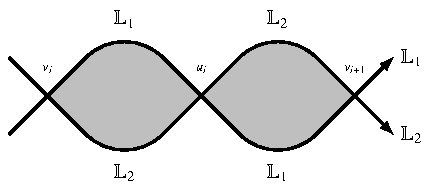
\includegraphics[width=0.72\textwidth]{figures/Fig_068_PDF153_Book141.pdf}
  \caption{圆柱上两条拉格朗日曲线的交点与次数（原书 p.141）}
  \label{fig:cylinder-lagrangians-intersections}
\end{figure}

从某个 $u$ 到相邻的 $v$ 恰有一条全纯条带。后一侧的条带带正号，前一侧的条带带负号：
\[
  CF_k^{\pm}(L_1,L_2)=\bigoplus_{i=1}^r(ku_i\oplus kv_i),
  \qquad \mu_1(u_i)=v_{i+1}-v_i.
\]
该复形的上同调由 $\iota=\sum_i u_i$ 与 $\xi=v_1$ 张成（在上同调中也可以用任意 $v_i$ 代替 $v_1$，因为它们彼此相等）。转到极小模型后，对每一对横截曲线都有
\[
  H\widehat{\mathrm{Fuk}}^{\pm}(L_1,L_2)
  =k\iota^{[12]}\oplus k\xi^{[12]}.
\]

为了将这个预范畴范畴化，注意每个 $\iota^{[12]}$ 都是拟同构。事实上，若 $u^{[13]}\colon L_1\to L_3$ 是一个零次交点，它恰好位于一个由零次交点构成的三角形中；该三角形由 $L_1$ 上先于它的 $u^{[12]}$ 和 $L_2$ 上后于它的 $u^{[23]}$ 张成，或者在 $L_2$ 位于 $u^{[13]}$ 上方或下方时反过来。因此有
\[
  \iota^{[23]}\iota^{[12]}=\iota^{[13]}.
\]
\begin{figure}[H]\centering
  \centering
  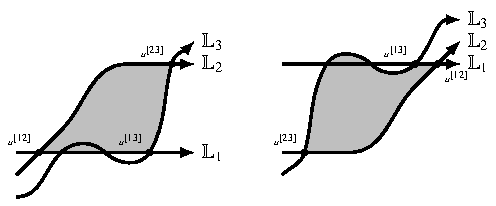
\includegraphics[width=0.74\textwidth]{figures/Fig_069_PDF154_Book142.pdf}
  \caption{零次交点的三角形乘积（原书 p.142）}
  \label{fig:cylinder-triangle-product}
\end{figure}
类似地，可以推出
\[
  \xi^{[23]}\iota^{[12]}=\iota^{[23]}\xi^{[12]}=\xi^{[13]},
  \qquad \xi^{[23]}\xi^{[12]}=0.
\]
范畴化之后，定向相同的所有对象都彼此同构，所有 $\iota$ 都成为单位。经过一次 $A_\infty$ 同构，可以把它们化为严格单位。这意味着，可能非零的高阶乘积只涉及 $\xi$。然而，若考察由同一方向绕圆柱的拉格朗日子流形围成的任意 $n$ 边形，它们不可能都沿着多边形的同一方向行进。于是至少有两处方向发生改变，这两处中至少一处会在乘积中出现为一个 $\iota$，因此
\[
  \mu(\xi,\ldots,\xi)=0.
\]
\begin{figure}[H]\centering
  \centering
  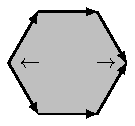
\includegraphics[width=0.28\textwidth]{figures/Fig_070_PDF154_Book142.pdf}
  \caption{沿圆柱同向绕行的多边形必有方向转折（原书 p.142）}
  \label{fig:cylinder-polygon-direction}
\end{figure}

由此可知，Fukaya 范畴等价于一个普通的 $\mathbb Z_2$-分次范畴，它有两个对象 $\{L_+,L_-\}$，且
\[
  \begin{aligned}
  \widehat{\mathrm{Fuk}}^{\pm}(L_+,L_+)
  &=\widehat{\mathrm{Fuk}}^{\pm}(L_-,L_-)
   =k[\xi]/(\xi^2)=\Lambda_1^{\pm},\\
  \widehat{\mathrm{Fuk}}^{\pm}(L_+,L_-)
  &=\widehat{\mathrm{Fuk}}^{\pm}(L_-,L_+)
   =k[\xi]/(\xi^2)[1]=\Lambda_1^{\pm}[1].
  \end{aligned}
\]
取导出版本，则
\[
  D\widehat{\mathrm{Fuk}}^{\pm}(X,\theta,J)\cong_\infty D\Lambda_1^{\pm}.
\]
\end{example}

\subsection{提升分次}\label{subsec:upgrade-grading}
在前面的构造中，我们只给范畴赋予了 $\mathbb Z_2$-分次，但有时也可以构造 $\mathbb Z$-分次范畴。理想情况下，要全面讨论 Fukaya 范畴的分次，应当介绍 Maslov 指数\bookcite{12,173,238}；它是 Floer 理论中 Morse 指数的推广。不过，这里我们采用与第~\ref{subsec:morse-dynamics} 节一致的较基础方法。

\begin{definition}{Calabi--Yau 流形}{calabi-yau-manifold}
Calabi--Yau 流形\index{calabiyauliuxing@Calabi–Yau 流形|hyperpage} $(X,\Omega)$ 是一个 Kähler 流形 $(X,\omega,J)$，配有处处不为零的复体积形式 $\Omega\in\Omega^n_{\mathbb C}(X)$。
\end{definition}

与第~\ref{subsec:morse-dynamics} 节的讨论类似，可以利用这个体积形式定义分次拉格朗日子流形\index{fencilagelangriziliuxing@分次拉格朗日子流形|hyperpage}，并给 Floer 复形赋予分次。

\begin{definition}{$\Omega$-分次拉格朗日子流形}{omega-graded-lagrangian}
$\Omega$-分次拉格朗日子流形是一个二元组 $(L,\theta)$，其中 $L$ 是拉格朗日子流形，$\theta\colon L\to\mathbb R$ 是函数，并且 $e^{-i\theta}\Omega$ 是 $L$ 上的实体积形式。若 $L$ 可由常值函数赋予分次，则称它为特殊拉格朗日子流形\index{teshulagelangriziliuxing@特殊拉格朗日子流形|hyperpage}。
\end{definition}

并非每个拉格朗日子流形都可以赋予分次。对每个 $x\in L$，$\theta(x)$ 都只确定到相差 $\pi$ 的整数倍。若在 $x$ 处固定 $\theta$，并沿曲线 $\gamma\colon x\to y$ 延拓，就能得到 $\theta(y)$；要使 $L$ 可分次，这个延拓结果必须与路径选择无关。若 $L$ 连通且可分次，那么每个 $k\in\mathbb Z$ 恰好对应一个分次，因为两个分次全局相差 $\pi$ 的整数倍。分次会自动给拉格朗日子流形定向：取 $e^{-i\theta}\Omega$ 作为实体积形式即可。相差奇数倍 $\pi$ 的两个分次给出相反定向。

\begin{definition}{分次交点的次数}{graded-intersection-degree}
设两个带分次的拉格朗日子流形 $(L_1,\theta_1)$ 和 $(L_2,\theta_2)$ 在 $x$ 处横截相交。取一个相对于几乎复结构 $J$ 的酉映射 $U\colon T_xX\to T_xX$，使得 $U(T_xL_1)=T_xL_2$，并选取 $\Delta\in[0,\pi)$ 使 $\det U=\pm e^{i\Delta}$。定义 Floer 复形 $CF_k^\bullet(L_1,L_2)$ 中交点 $x$ 的次数为
\[
  \deg x=\frac{\Delta-(\theta_2(x)-\theta_1(x))}{\pi}.
\]
\end{definition}

\begin{lemma}{分次交点次数与乘积次数}{graded-fukaya-product-degree}
交点 $x$ 的次数定义良好，且乘积 $\mu_k$ 的次数为 $2-k$。
\end{lemma}
\begin{proof}[证明梗概]
首先，$\deg x$ 是整数，因为
$U^*(\Omega|_{T_xL_2})=\det(U)\,\Omega|_{T_xL_1}$，从而
$\Delta-(\theta_2(x)-\theta_1(x))$ 是 $\pi$ 的整数倍。其定义也与 $U$ 的选取无关，因为 $U$ 只在左右乘上固定 $T_xL_1$ 或 $T_xL_2$ 的酉变换时才会改变；这些变换在对应子空间上都是正交变换，故行列式为 $\pm1$。

为了求 $\mu_k$ 的次数，可以把每个伪全纯映射的定义域从圆盘变换为内角为相应 $\Delta$ 的凸多边形。结论便由 $k$ 边形内角和为 $(k-2)\pi$ 得出。
\end{proof}
% [Tutor Note: $\Delta$ 取的是 Maslov 指数模 $\pi$ 的代表元：公式给出 $\mathbb Z$-次数，模 $2$ 即得先前的 $\mathbb Z_2$-次数。$U$ 只确定到左乘、右乘分别固定 $T_xL_1$、$T_xL_2$ 的正交变换，其行列式为 $\pm1$，故 $\Delta$ 的模 $\pi$ 约化与 $\deg x$ 均与 $U$ 的选取无关；实际计算时务必先固定 $L_1,L_2$ 的定向与分次。]

\begin{definition}{整数分次基本 Fukaya 范畴}{z-graded-basic-fukaya}
$\mathbb Z$-分次基本 Fukaya 预范畴 $\widehat{\mathrm{Fuk}}^\bullet(X,\Omega)$ 的横截序列，由满足以下条件的 $\Omega$-分次拉格朗日子流形组成：它们两两横截相交、紧致、正合，并带有自旋结构；其 Hom 空间是相应的 $\Omega$-分次 Floer 复形，乘积则仍按前述方式定义。$\mathbb Z$-分次 Fukaya 范畴 $\widehat{\mathrm{Fuk}}^\bullet(X,\Omega)$ 是该预范畴的范畴化。
\end{definition}

整数分次 Fukaya 预范畴依赖于 $\Omega$，但不同的 $\Omega$ 也可能给出同构范畴。若存在一条由复体积形式构成的路径连接 $\Omega_0$ 与 $\Omega_1$，就称它们同伦。

\begin{lemma}{同伦复体积形式给出同构预范畴}{homotopic-volume-forms}
同伦的复体积形式诱导同构的 Fukaya 预范畴。
\end{lemma}
\begin{proof}[证明梗概]
设 $\Omega_t$（$t\in[0,1]$）是连接两者的路径。对每个点 $x$，可以计算 $\Omega_t(x)$ 的相位沿该路径变化了多少：
\[
  \vartheta(x)=\int_0^1d\arg\Omega_t(x).
\]
若 $\theta\colon L\to\mathbb R$ 是 $\Omega_0$-分次，那么 $\theta-\vartheta$ 就是 $\Omega_1$-分次，反之亦然。因此，$\Omega_0$-分次与 $\Omega_1$-分次拉格朗日子流形之间存在双射。由这些分次诱导的 Floer 复形分次相同，因为相位项 $\vartheta$ 会相消。
\end{proof}

\begin{example}[圆柱上的整数分次]
利用坐标 $z=e^{p+qi}$，可以把 $X=T^*S^1$ 识别为 $\mathbb C^*$。复体积形式是处处不为零的 $1$-形式，例如 $\Omega=z^r\,dz$。要给底拉格朗日子流形 $S^1$ 赋予分次，必须取
\[
  \theta(q)=-rq-q+k\pi.
\]
除非 $r=-1$，否则该函数不具周期性，因此不是定义在圆上的函数。

这意味着，除非 $\Omega=dz/z$，整数分次基本 Fukaya 范畴为空。在此情形下，它等价于一个对象为 $L[k]$（$k\in\mathbb Z$）的范畴；这些对象对应分次拉格朗日子流形 $(S^1,k\pi)$，且
\[
  \widehat{\mathrm{Fuk}}^\bullet(L[i],L[j])
  =k[\xi]/(\xi^2)[j-i]=\Lambda_1^\bullet[j-i].
\]
在导出层面可得
\[
  D\widehat{\mathrm{Fuk}}^\bullet\left(\mathbb C^*,\frac{dz}{z}\right)
  \cong_\infty D\Lambda_1^\bullet\cong_\infty D\mathrm{mod}^\bullet k[[X]].
\]
\end{example}

\section{变体}\label{sec:fukaya-variations}
现在构造一些 Fukaya 型范畴，它们是前一构造的不同变体。每个变体都有两种版本：若存在复体积形式 $\Omega$，则有 $\mathbb Z$-分次版本；否则只有 $\mathbb Z_2$-分次版本。为避免重复和记号繁杂，下文省略 $\Omega$，但范畴记号采用 $\mathbb Z$-分次版本。

\takeaway{基本构造可扩充为多种变体：纳入浸入与局部系统；用 Reeb 弦与带结的圆盘定义 wrapped Fukaya 范畴；用 stop 截断 Reeb 流得到 partially wrapped 范畴；以 Lefschetz 纤维化的 thimble 定义有向 Fukaya 范畴；并借除子与 Novikov 域处理紧致流形的相对与完整 Fukaya 范畴。}

\subsection{浸入与局部系统}\label{subsec:immersions-local-systems}
可以从两个方向扩充 Floer 上同调的适用范围：允许拉格朗日子流形是浸入的，并在拉格朗日子流形上配置局部系统。

\begin{definition}{带局部系统的浸入拉格朗日子流形}{lagrangian-brane}
带局部系统的浸入拉格朗日子流形（也称拉格朗日膜\index{lagelangrimo@拉格朗日膜|hyperpage}）是三元组 $(L,\mathcal L,\phi)$，其中：
\begin{itemize}
  \item $L$ 是一个 $n$ 维紧致定向流形（若 $\operatorname{char}k\ne2$，还须带有自旋结构）；
  \item $\mathcal L\colon\Pi_1(L)\to\mathrm{vect}(k)$ 是一个局部系统；
  \item $\phi\colon L\to X$ 是浸入，且对所有 $p\in L$，$\phi_*T_pL$ 都是拉格朗日子空间。
\end{itemize}
此外，我们要求浸入的自交是横截的：$L$ 中至多两个点映到 $X$ 中的同一点；若 $\phi(p_1)=\phi(p_2)=x$，则
\[
  T_xX=\phi_*T_{p_1}L\oplus\phi_*T_{p_2}L.
\]
这样的点称为双点。若存在 $f\colon L\to\mathbb R$ 使 $\phi^*\theta=df$，则称该浸入正合。
\end{definition}

若正合拉格朗日膜 $L_i:=(L_i,\mathcal L_i,\phi_i)$ 两两横截相交，且交点不是双点，则可定义 Floer 复形
\[
  CF_k^\bullet(L_1,L_2)=
  \bigoplus_{p\in\phi_1(L_1)\cap\phi_2(L_2)}
  \mathrm{Hom}_k\!\left(\mathcal L_1(\phi_1^{-1}p),
                        \mathcal L_2(\phi_2^{-1}p)\right)\,p.
\]
乘积变为
\[
  \begin{aligned}
  \mu(\alpha_1p_1,\ldots,\alpha_kp_k)
  :=\sum_{p_0\in\phi_0(L_0)\cap\phi_k(L_k)}\sum_\psi
  &\mathcal L_0(\gamma_0)\alpha_1\mathcal L_1(\gamma_1)\cdots
   \alpha_k\mathcal L_k(\gamma_k)\,\epsilon_\psi\,p_0.
  \end{aligned}
\]
这里 $\gamma_r$ 表示将伪全纯圆盘边界拉回到 $L_r$ 后、从 $p_{r+1}$ 到 $p_r$ 的路径：
\[
  \gamma_r\colon[0,1]\to L_r,\qquad
  t\longmapsto\phi_r^{-1}\psi\!\left(e^{\frac{2(r+1-t)\pi i}{k+1}}\right).
\]

\begin{figure}[H]\centering
  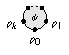
\includegraphics[width=0.25\textwidth]{figures/Fig_071_PDF157_Book145.pdf}
  \caption{浸入圆盘边界上的平行移动（原书 p.145）}
  \label{fig:brane-disk-transport}
\end{figure}
换言之，Floer 复形中的元素变成了交点处纤维之间的态射，而乘积则记录沿浸入圆盘边界的平行移动。线性映射 $\mathcal L_i(\gamma_i)$ 只依赖路径的同伦类，因此因子 $\mathcal L_0(\gamma_0)\alpha_1\mathcal L_1(\gamma_1)\cdots\alpha_k\mathcal L_k(\gamma_k)$ 在 $\psi$ 形变或退化时保持不变。这一点对 $A_\infty$ 公理中的各项相消至关重要。

在这一推广设定下，只要把 $\phi_\epsilon^h(L)$ 理解为 $(L,\mathcal L,\phi_\epsilon^h\circ\phi)$，Floer 理论的主定理仍然成立。把普通拉格朗日子流形 $L$ 视为带平凡一维局部系统的膜，就能恢复原来的 Floer 理论：对任意点 $p$ 和曲线 $\gamma$，有 $\mathcal L(p)=k$、$\mathcal L(\gamma)=1$。

局部系统的思想还可以用来描述 $L$ 上的不同自旋结构。给定 $L$ 上一个自旋结构，所有其他自旋结构可由 $H^1(L,\mathbb Z_2)$ 参数化。这个空间也可识别为所有满足如下条件的局部系统 $\mathcal S$：$\mathcal S(p)$ 为一维，且对任意闭路 $\gamma$，$\mathcal S(\gamma)=\pm1$。拉格朗日膜 $(L,\mathcal S,\phi)$ 因而可以解释为带有另一种自旋结构的同一个拉格朗日子流形。

\begin{definition}{正合 Fukaya 范畴}{exact-fukaya-category}\index{zhenghefukayafanchou@正合 Fukaya 范畴|hyperpage}
正合 Fukaya 预范畴 $\mathrm{exFuk}^\bullet(X)$ 的横截序列由两两横截相交且交点彼此不同的正合拉格朗日膜组成，乘积按上文定义。正合 Fukaya 范畴 $\mathrm{exFuk}^\bullet(X)$ 定义为相应预范畴的范畴化。
\end{definition}

\begin{example}[圆的余切丛上的局部系统与浸入]
回到带有 $\Omega=dz$ 的圆的余切丛 $T^*S^1=\mathbb C^*$。

\textbf{局部系统。} 为描述 $S^1$ 上的局部系统 $\mathcal L$，先选取基点 $b\in S^1$，并在 $\mathcal L(b)$ 中选一组基。这给出矩阵 $M=\mathcal L(\ell)$，其中 $\ell$ 是以 $b$ 为基点、沿正向绕圆一周的环路。该局部系统对应表示
\[
  \rho_M\colon\pi_1(S^1)\to\mathrm{GL}_n,
  \qquad \ell^k\longmapsto M^k.
\]
对每个其他点 $x$，从 $b$ 沿正向到 $x$ 有一条唯一的最短路径（按同伦类计）。可以选择 $\mathcal L(x)$ 中的基，使沿该路径的平行移动为恒等映射。固定这些基后，$\mathcal L(\gamma)=M^k$，其中 $k$ 是 $\gamma$ 沿正向穿过 $b$ 的次数减去沿反向穿过 $b$ 的次数。

现在考虑两个嵌入的、正合且正向定向的拉格朗日子流形 $L_1,L_2$，它们分别带有局部系统 $\mathcal L_1,\mathcal L_2$，对应矩阵为 $M_1,M_2$。若交点为 $u_i,v_i$（$1\le i\le r$），并假设两个基点都位于 $u_r$ 与 $v_1$ 之间，则 Floer 复形为
\[
  CF(L_1,L_2)=\bigoplus_{i=1}^r
  \left(\mathrm{Mat}_{n_2\times n_1}(k)u_i\oplus
        \mathrm{Mat}_{n_2\times n_1}(k)v_i\right),
\]
其中当 $i\ne r$ 时，
\[
  \mu_1(Au_i)=Av_{i+1}-Av_i,
\]
而绕过基点的最后一项为
\[
  \mu_1(Au_r)=M_2AM_1^{-1}v_1-Av_r.
\]
该复形的上同调可解释为
\[
  \operatorname{Ext}_{\pi_1(S^1)}^\bullet(\rho_{M_1},\rho_{M_2}).
\]
因此，允许局部系统后，Fukaya 范畴的行为类似于有限维 $\pi_1(S^1)$-模范畴。

\textbf{浸入。} 圆的一个浸入形如 $\phi\colon t\mapsto(kt,p(t))$，其中 $k\in\mathbb Z$ 是绕数，$p(t)$ 是 $2\pi$-周期函数。若 $p$ 是某个 $2\pi$-周期原函数 $f$ 的导数，该浸入就是正合的。

比较底圆 $L_1=S^1\subset T^*S^1$ 上由 $M_1\in\mathrm{Mat}_{2\times2}(k)$ 决定的二维局部系统，与绕圆柱两周、带有传递矩阵 $M_2\in k$ 的一维局部系统的浸入拉格朗日子流形。此时
\begin{figure}[H]\centering
  \centering
  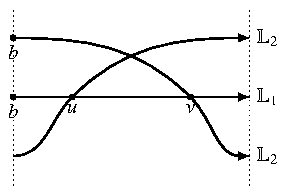
\includegraphics[width=0.54\textwidth]{figures/Fig_072_PDF159_Book147.pdf}
  \caption{嵌入圆与绕圆柱两周的浸入（原书 p.147）}
  \label{fig:immersed-circle-local-system}
\end{figure}
\[
  CF(L_1,L_2)=k^2u\oplus k^2v,
  \qquad
  \mu_1(Au)=M_1Av-M_1^{-1}AM_2^{-1}v.
\]
若 $M_1^2=M_2I_2$，该微分为零，因而有两个非零零次态射。进一步考察可知，若 $M_1=\begin{pmatrix}0&M_2\\1&0\end{pmatrix}$，则这两个对象同构。直观上，这是合理的：此时 $L_1$ 上的局部系统是沿投影 $L_2\to L_1$ 拉回 $L_2$ 上局部系统所得。

利用这一思想可以证明：任何绕圆柱 $n$ 圈、带有 $k$ 维局部系统的浸入拉格朗日子流形，都与一个嵌入拉格朗日子流形及其上的 $nk$ 维局部系统同构。

\textbf{多个连通分支。} 还可以浸入多个连通分支。此时 $L=L_1\sqcup\cdots\sqcup L_k$，浸入与局部系统在每个分支上的限制都可视为 Fukaya 范畴中的独立对象。不难证明，在加法完备化中，大对象同构于各小对象的直和：
\[
  (L,\phi,\mathcal L)\cong
  \bigoplus_i(L_i,\phi|_{L_i},\mathcal L|_{L_i}).
\]
\end{example}

从这一讨论可见，Fukaya 范畴中的对象是带局部系统的分次圆的直和。每个对象都等价于 $\pi_1(S^1)$ 或其群环 $k[X,X^{-1}]$ 上有限维模的某个移位。与多项式环的情形类似，导出范畴 $D\mathrm{mod}^\bullet k[X,X^{-1}]$ 中的每个对象都具有这种形式，因此
\[
  \mathrm{exFuk}^\bullet(X)\cong_\infty D\mathrm{mod}^\bullet k[X,X^{-1}].
\]
从这一角度看，同时纳入浸入与局部系统是很自然的。这样得到的 Fukaya 范畴性质更好，因为它对直和、移位乃至锥封闭。因此，下文所说的 Fukaya 范畴一律指这个版本，而不是最初构造的基本版本。

\subsection{wrapped Fukaya 范畴}\label{subsec:wrapped-fukaya}
在上一个例子中，我们看到，圆的余切丛的 Fukaya 范畴可以识别为 $\pi_1(S^1)$ 的有限维表示所成的 $A_\infty$ 范畴。从表示论角度看，若还能纳入一些良好的无限维模（例如有限生成投射模），会更理想。为此，我们应当在 Fukaya 范畴的构造中纳入非紧致拉格朗日子流形；显然可以选择具有锥形端的子流形。

从带柱状端、配有相容几乎复结构的 Liouville 流形 $(X,\theta,J)$ 出发。在 $X$ 上选取 Hamilton 函数 $h\colon X\to\mathbb R$，令它在 Liouville 域 $X_0$ 上为零，并在柱体的向外坐标 $r$ 上呈二次增长。该 Hamilton 函数生成的流称为 Reeb 流\index{reebliu@Reeb 流|hyperpage}，其流线
\[
  \gamma_x\colon[0,1]\to X,\qquad t\longmapsto\phi_t^h(x)
\]
称为 Reeb 弦\index{reebxian@Reeb 弦|hyperpage}。Reeb 流保持坐标 $r$ 不变，因此每条 Reeb 弦都在某个 $\partial X_0\times\{r\}$ 上绕行。随着 $r$ 增大，由于 $h$ 关于 $r$ 是二次的，Reeb 弦绕行得越来越快。

\begin{definition}{wrapped Floer 复形}{wrapped-floer-complex}
若 $L_1,L_2$ 是正合拉格朗日子流形，且 $\phi_1^hL_1$ 与 $L_2$ 横截相交，则 wrapped Floer 复形 $CW(L_1,L_2;h)$ 定义为由连接 $L_1$ 与 $L_2$ 的 Reeb 弦张成的向量空间：
\[
  CW(L_1,L_2;h)=
  \bigoplus_{\substack{\gamma(0)\in L_1\\\gamma(1)\in L_2}}k\gamma.
\]
\end{definition}

作为向量空间，该复形与 $CF^{\pm}(\phi_1^hL_1,L_2)$ 同构，因为每条 Reeb 弦都对应一个交点。利用这一识别，可以给 $CW(L_1,L_2;h)$ 赋予 $\mathbb Z_2$-分次；若 $X$ 是 Calabi--Yau 流形，还可以赋予 $\mathbb Z$-分次。
\begin{figure}[H]\centering
  \centering
  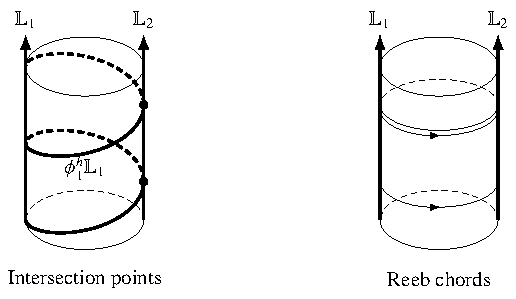
\includegraphics[width=0.79\textwidth]{figures/Fig_073_PDF161_Book149.pdf}
  \caption{交点与 Reeb 弦的对应（原书 p.149）}
  \label{fig:wrapped-intersections-chords}
\end{figure}

乘积仍通过统计浸入圆盘来定义，但此时会遇到配对问题。若 Reeb 弦 $\gamma_1$ 对应于 $\phi_1^hL_0$ 与 $L_1$ 之间的交点 $p_1$，而 Reeb 弦 $\gamma_2$ 对应于 $\phi_1^hL_1$ 与 $L_2$ 之间的交点 $p_2$，那么 $L_1$ 与 $\phi_1^hL_1$ 并不重合。可以把 $p_1$ 沿流推到交点 $\phi_1^hp_1$，它属于 $\phi_2^hL_0$ 与 $\phi_1^hL_1$ 的交点。但若以 $p_2$ 和 $\phi_1^hp_1$ 为角点统计三角形，第三个角点将落在 $\phi_2^hL_0$ 与 $L_2$ 的交点中。由于 $\phi_2^hL_0=\phi_1^{2h}L_0$，这对应于 $CW(L_0,L_2;2h)$ 中的一条 Reeb 弦。

因此，乘积 $\widetilde\mu_k$ 是映射
\[
  \widetilde\mu_k\colon
  CW(L_{k-1},L_k;h)\otimes\cdots\otimes CW(L_0,L_1;h)
  \longrightarrow CW(L_0,L_k;kh).
\]
用 Reeb 弦表述，它统计如下对象。设 $\gamma_i\in CW(L_{i-1},L_i;h)$（$i=1,\ldots,k$）是 Reeb 弦，且 $\gamma_0\in CW(L_0,L_k;kh)$。令 $D_{k+1}$ 为去掉 $k+1$ 段圆周弧后的闭单位圆盘：
\[
  D_{k+1}=D\setminus
  \bigcup_{i=0}^{k}\left\{
  e^{\frac{2t\pi i}{2k+2}}\ \middle|\ t\in(2i+1,2i+2)\right\}.
\]
考虑从 $D_{k+1}$ 到 $X$ 的映射 $\psi$，按重参数化取等价类，并要求：
\begin{itemize}
  \item 若 $t\in(2i,2i+1)$，则 $\psi(e^{\frac{2t\pi i}{2k+2}})\in L_i$；
  \item 若 $t\in(2i+1,2i+2)$、$i\in\{0,\ldots,k-1\}$，则当 $u\to e^{\frac{2t\pi i}{2k+2}}$ 时，$\psi(u)$ 的极限为 $\gamma_{i+1}(t-2i-1)$；
  \item 若 $t\in(2k+1,2k+2)$，则当 $u\to e^{\frac{2t\pi i}{2k+2}}$ 时，$\psi(u)$ 的极限为 $\gamma_0(2k+2-t)$；
  \item $\psi$ 满足一个经过变形的 Cauchy--Riemann 方程。
\end{itemize}
与原来一样，高阶乘积定义为所有不能再形变的这类映射之和。

为了得到真正的乘积，还应将 $\widetilde\mu_k$ 与映射
\[
  S_k\colon CW(L_0,L_k;kh)\to CW(L_0,L_k;h)
\]
复合。由于 $\phi_1^hL_0$ 与 $\phi_1^{kh}L_0$ Hamilton 同痕，这两个复形拟同构，所以可以选择 $S_k$ 为拟同构。要对所有可能的拉格朗日子流形自然地选取这些映射 $S_k$，并使 $\mu_k=S_k\widetilde\mu_k$ 满足 $A_\infty$ 关系，技术上相当复杂。细节可参见\bookcite{15,6}。
% [Tutor Note: 配对问题说明 $CW$ 上的乘积不能像 $CF$ 那样直接计数：$\phi_1^{kh}L_0$ 与 $\phi_1^hL_0$ 只是 Hamilton 同痕而非相等，故先用 $\widetilde\mu_k$ 落到 $CW(\cdot,\cdot;kh)$，再用拟同构 $S_k$ 拉回。原文未写出的是：这些 $S_k$ 还必须满足相干性条件（与 $\widetilde\mu$ 的复合在高阶上相容），否则 $\mu_k=S_k\widetilde\mu_k$ 不满足 $A_\infty$ 关系。]

若 $L_1,L_2$ 是包含于 Liouville 域 $X_0$ 中的紧致拉格朗日子流形，这一构造就退化为原来的构造，因为此时 $h|_{X_0}=0$，流为恒等映射。也可以像之前那样纳入浸入与局部系统。

\begin{definition}{wrapped Fukaya 范畴}{wrapped-fukaya-category}
wrapped Fukaya 预范畴 $\mathrm{wrFuk}^\bullet(X,h)$ 的对象是浸入的、正合的、带锥形端的拉格朗日子流形，其上配有自旋结构与局部系统，紧致子流形也在其中；Hom 空间是 wrapped Floer 复形 $CW^\bullet(L_0,L_1;h)$，乘积为上述 $\mu_k$。wrapped Fukaya 范畴\index{wrappedfukayafanchou@wrapped Fukaya 范畴|hyperpage} $\mathrm{wrFuk}^\bullet(X)$ 定义为该预范畴的范畴化。
\end{definition}

在 $A_\infty$ 拟等价意义下，$\mathrm{wrFuk}^\bullet(X)$ 与几乎复结构及 $h$ 的选取无关，并且有全忠实嵌入
\[
  \mathrm{exFuk}^\bullet(X)\hookrightarrow\mathrm{wrFuk}^\bullet(X).
\]

\begin{example}[圆的余切丛的 wrapped Fukaya 范畴]
回到 $T^*S^1$ 的例子。任意余切纤维 $L=T_x^*S^1$ 都是正合且带锥形端的拉格朗日子流形。每条 Reeb 弦 $\gamma$ 都由绕数 $w(\gamma)$ 决定；用 $X^{w(\gamma)}$ 表示它，就有
\[
  CW(L,L;h)\cong k[X,X^{-1}].
\]
对标准分次 $\Omega=dz/z$（取分次 $(L,\pi/2)$），所有 $X^i$ 的次数都是 $0$，所以唯一可能非零的乘积是 $\mu_2$。浸入圆盘的总绕数为零，因此非零乘积只能是
\[
  \mu(X^i,X^j)=X^{i+j}.
\]
下图在圆柱的万有覆盖上展示了相应的浸入：
\begin{figure}[H]\centering
  \centering
  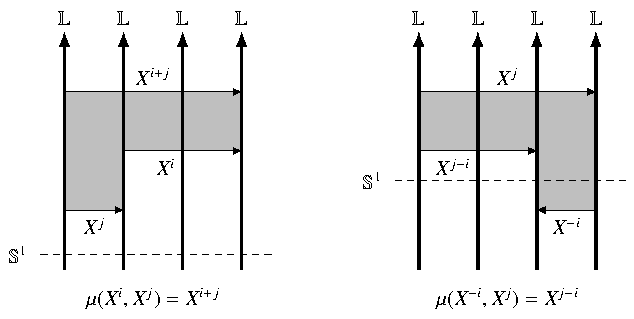
\includegraphics[width=0.88\textwidth]{figures/Fig_074_PDF163_Book151.pdf}
  \caption{$\mu(X^i,X^j)$ 与 $\mu(X^{-i},X^j)$ 的浸入圆盘（原书 p.151）}
  \label{fig:wrapped-circle-products}
\end{figure}

其他正合的锥形拉格朗日子流形可看成两条直线端由一条在底圆附近绕圆柱若干圈的曲线连接而成。若两端位于同一侧，则该对象是零对象，因为有 $1=d\gamma$，其中 $\gamma$ 是连接两端的最短 Reeb 弦。若两端位于相反侧，则该对象（取适当定向）同构于 $T^*S^1$。
\begin{figure}[H]\centering
  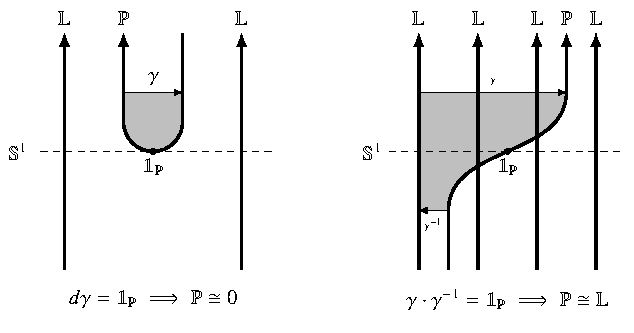
\includegraphics[width=0.79\textwidth]{figures/Fig_075_PDF163_Book151.pdf}
  \caption{由端点位置判定 wrapped 范畴中的对象（原书 p.151）}
  \label{fig:wrapped-circle-objects}
\end{figure}

因为 $L$ 可缩，其上的局部系统均为平凡局部系统；所有其他连通对象都同构于余切纤维的某个移位或直和。后者对应于自由 $k[X,X^{-1}]$-模。因此
\[
  \mathrm{wrFuk}^\bullet\left(X,\frac{dz}{z}\right)
  \cong_\infty D\mathrm{Mod}^\bullet k[X,X^{-1}].
\]
若选择分次形式 $\Omega=z^kdz$，其中 $k\ne-1$，仍可给余切纤维赋予分次，因为它是可缩的。态射 $X^i\in CW(L,L)\cong k[X,X^{-1}]$ 的次数为 $i(k+1)$。由于普通 Fukaya 范畴为空（不存在紧致对象），有
\[
  \mathrm{wrFuk}^\bullet(X,z^kdz)\cong_\infty Dk[X,X^{-1}],
  \qquad \deg X=k+1.
\]
% [Tutor Note: 原文 p.164 末作 $\deg X=k-1$，与同页上一行的“$X^i$ 的次数为 $i(k+1)$”矛盾，应为 $k+1$：由 $\Omega=z^kdz=z^{k+1}(dp+idq)$ 可见沿纤维绕行时相位按 $(k+1)$ 倍变化，故 $\deg X=k+1$。]
\end{example}

\begin{note}\label{note:wrapped-vs-ordinary-fukaya}
\textbf{观察 6.48.} wrapped Fukaya 范畴与普通 Fukaya 范畴之间的关系，类似于有限维模的导出范畴与有限生成模范畴之间的关系。
\end{note}

\subsection{partially wrapped Fukaya 范畴}\label{subsec:partially-wrapped-fukaya}
设 $(X,\theta)$ 是带柱状端的 Liouville 流形。一般而言，柱体上的 Reeb 流会使锥形拉格朗日子流形的自同态空间变成无限维。在某些情形下这是我们想要的，但另一些情形中它会带来不便。因此，我们引入一种中断该流的方法。

\begin{definition}{stop}{fukaya-stop}
设 $U_0$ 是 $\partial X_0$ 中的一个超曲面，并令 $U:=U_0\times[1,\infty)$。它构成 $X$ 的柱状端中的超曲面；若 Reeb 流处处与该超曲面法向，则称 $U$ 为 stop\index{stop@stop|hyperpage}。
\end{definition}

由于 Reeb 流处处与超曲面法向，Reeb 弦只能沿一个方向穿过它。因此，可以把 Reeb 弦的 $U$-次数定义为它穿过 $U$ 的次数。

\begin{lemma}{wrapped Fukaya 范畴中的乘积不增加 stop 次数}{stop-degree-monotonicity}
对与 $U$ 不相交的拉格朗日子流形，wrapped Fukaya 范畴中的乘积不会增加 $U$-次数。也就是说，若
\[
  \mu_k(\gamma_1,\ldots,\gamma_k)=\sum_i\alpha_i\zeta_i,
\]
则 $\zeta_i$ 的 $U$-次数至多为各 $\gamma_i$ 的 $U$-次数之和。
\end{lemma}
\begin{proof}[证明梗概]
考察由 $\gamma_i$ 围成的浸入圆盘 $\psi\colon D\to X$，其边界上还有一条输出弦 $\zeta$。原像 $\psi^{-1}(U)$ 是一族带定向曲线。这些曲线只能从 $\gamma_i$ 进入、从 $\zeta_i$ 离开，因为只有 $\zeta_i$ 在圆盘边界上的方向与之相反。
\begin{figure}[H]\centering
  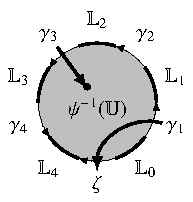
\includegraphics[width=0.44\textwidth]{figures/Fig_076_PDF165_Book153.pdf}
  \caption{圆盘中 stop 的原像曲线（原书 p.153）}
  \label{fig:stop-preimage-curves}
\end{figure}
若全纯圆盘有一部分位于柱体之外，这些曲线也可以在 $\psi^{-1}(U_0)$ 中的点处终止。
\end{proof}

\begin{definition}{partially wrapped Fukaya 范畴}{partially-wrapped-fukaya-category}
设 $\sigma$ 是一组可能彼此相交的 stop。partially wrapped Fukaya 预范畴 $\mathrm{wrFuk}^\bullet_\sigma(X)$ 的对象，是 wrapped Fukaya 范畴中与所有 $U\in\sigma$ 不相交的对象；其态射空间由 wrapped Fukaya 范畴中对每个 $U\in\sigma$ 的 $U$-次数均为 $0$ 的态射组成。partially wrapped Fukaya 范畴\index{partiallywrappedfukayafanchou@partially wrapped Fukaya 范畴|hyperpage} $\mathrm{wrFuk}^\bullet_\sigma(X)$ 定义为该预范畴的范畴化。
\end{definition}

\begin{example}[圆的余切丛上的 stop]
仍考察圆的余切空间。此时 $X_0$ 是两个圆的不交并，$U_0$ 是这些圆上的一组选定点。
% [Tutor Note: 原文 p.165 此处作“$X_0$ 是两个圆的不交并”，疑为笔误：$X_0=\{x\in T^*S^1\mid\|p\|\le1\}$ 是圆柱 $S^1\times[-1,1]$，不交并的两个圆是其边界 $\partial X_0$；紧接着的 $U_0$ 也是 $\partial X_0$ 上的点。]
每个点都会在圆柱上确定一条向外延伸的射线。这些射线把上、下两端分成不同扇区，不同扇区之间没有 Reeb 弦。
\begin{figure}[H]\centering
  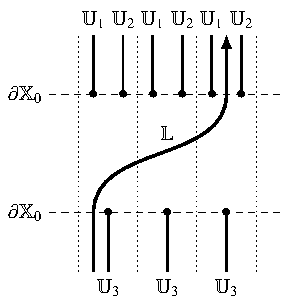
\includegraphics[width=0.86\textwidth]{figures/Fig_077_PDF165_Book153.pdf}
  \caption{圆柱端上的 stop 与扇区（原书 p.153）}
  \label{fig:stops-cylinder-sectors}
\end{figure}
锥形拉格朗日子流形由起始扇区、终止扇区及中间绕行的圈数决定。同一类型的子流形都给出同构对象。注意，在圆柱同一侧起始和终止、但处于不同扇区的对象，在 partially wrapped Fukaya 范畴中是非零对象；若移除 stop，这些对象在 fully wrapped 范畴中就变成零对象。现在考察三种特殊情形。

\begin{itemize}
  \item 若只有一个 stop（设在圆柱下端），则在同痕意义下只有一个非紧致拉格朗日子流形。它的自同态环为 $k[X]$，因为 $X$ 的所有负次幂都被 stop 消去。因此
  \[
    \mathrm{wrFuk}^\bullet_\sigma(X)\cong_\infty D\mathrm{Mod}^\bullet k[X].
  \]
  \item 若同一端有 $n$ 个 stop，则有 $n$ 条从底端通到顶端的不同拉格朗日子流形，它们的自同态环是循环箭图的路径代数。此外，对每个扇区和每个 $k$，还有一条拉格朗日子流形从顶端出发，先在 $X_0$ 中向右移动 $k$ 个扇区，再向上延伸；最后还要纳入紧致拉格朗日子流形。对照第 4.2.3 与 4.3.1 节可得
  \[
    \mathrm{wrFuk}^\bullet_\sigma(X)\cong_\infty
    D\mathrm{Mod}^\bullet\bigl(k[X]\star\mathbb Z_n\bigr).
  \]
  \item 若两端各有一个 stop，对照第 4.4.1 节可知，该范畴等价于下图所示单箭头箭图的模范畴导出范畴：
  \begin{figure}[H]\centering
    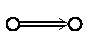
\includegraphics[width=0.13\textwidth]{figures/Fig_078_PDF166_Book154.pdf}
    \caption{单箭头箭图（原书 p.154）}
    \label{fig:single-arrow-quiver}
  \end{figure}
\end{itemize}

给定 Liouville 流形 $X$ 和一组 stop $\sigma$，由预范畴的自然嵌入给出一个 $A_\infty$ 函子
\[
  \mathrm{wrFuk}^\bullet_\sigma(X)\longrightarrow\mathrm{wrFuk}^\bullet(X).
\]
在以上每个例子中，这个函子实际上是一个局部化：一种将某个给定子范畴中的所有态射取为可逆态射的泛构造。在第一个例子中，我们把所有 $X$ 的正次幂取为可逆态射。这些态射恰好是其锥（余核）为幂零 $k[X]$-模的态射；换言之，它们是有限维 $k[[X]]$-模。因此可以写成
\[
  D\mathrm{Mod}^\bullet k[X,X^{-1}]
  \cong_\infty\frac{D\mathrm{Mod}^\bullet k[X]}{D\mathrm{mod}^\bullet k[[X]]}.
\]
partially wrapped Fukaya 范畴、移除 stop 与局部化的关系，见\bookcite{236,96}。
\end{example}

\subsection{有向 Fukaya 范畴}\label{subsec:directed-fukaya}
有向 Fukaya 范畴\index{youxiangfukayafanchou@有向 Fukaya 范畴|hyperpage}是为 Landau--Ginzburg 模型\index{landauginzburgmoxing@Landau–Ginzburg 模型|hyperpage}定义的 Fukaya 范畴。1998 年，Kontsevich 提出用这类模型研究 Fano 簇的镜像对称\bookcite{142}。其辛几何由有向 Fukaya 范畴捕捉，该范畴也称为 Fukaya--Seidel 范畴。Seidel 在其专著\bookcite{218}中详细阐述了构造；Abouzaid\bookcite{5}的工作给出略有不同的方法，并建立了它与环面 Fano 簇镜像对称之间的联系。

\begin{definition}{Landau--Ginzburg 模型}{landau-ginzburg-model}
Landau--Ginzburg 模型是一个二元组 $(X,W)$，其中 $X=(X,\theta,J)$ 是正合 Kähler 流形，$W\colon X\to\mathbb C$ 是全纯映射。
\end{definition}

可以取 $X=\mathbb C^n$，坐标 $z_i=p_i+iq_i$，并令 $\theta=p_i\,dq_i$；但更复杂的例子（例如带柱状端的 Liouville 流形）也适用。

\begin{definition}{临界点与 Lefschetz 纤维化}{lefschetz-fibration}
若在某组局部复坐标下，$W$ 的所有一阶偏导数都在 $p\in X$ 处为零，则称 $p$ 为临界点\index{linjiedian@临界点|hyperpage}。$W(p)$ 称为临界值\index{linjiezhi@临界值|hyperpage}。若 Hessian 矩阵 $\partial_{z_i}\partial_{z_j}W(p)$ 非退化，则称临界点非退化。若 $W$ 只有有限多个临界点 $\{p_1,\ldots,p_k\}$，且它们都非退化，则称 $W\colon X\to\mathbb C$ 为 Lefschetz 纤维化\index{lefschetzxianweihua@Lefschetz 纤维化|hyperpage}。
\end{definition}

Lefschetz 纤维化是 Morse 函数的复几何对应物，但二者的表现相当不同。与实情形不同，复 Hessian 总能化为单位矩阵，因此没有指标的概念。此外，Morse 函数在临界值两侧的纤维一般不同，但 Lefschetz 纤维化中所有非临界值的纤维彼此同构。
\begin{figure}[H]\centering
  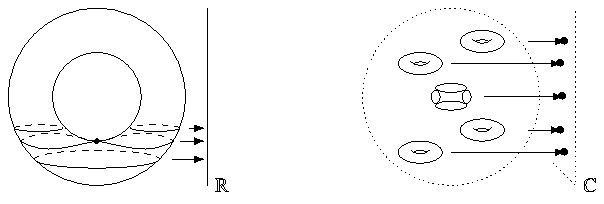
\includegraphics[width=0.38\textwidth]{figures/Fig_079_PDF167_Book155.pdf}
  \caption{Lefschetz 纤维化的正则纤维（原书 p.155）}
  \label{fig:lefschetz-regular-fibers}
\end{figure}

这是因为任意两个非临界值 $b,c$ 都可以由一条避开临界值的路径连接。取这样的路径 $\gamma\colon[0,1]\to\mathbb C$，满足 $\gamma(0)=b,\gamma(1)=c$。选择光滑函数 $h\colon\mathbb C\to\mathbb R$，令它沿 $\gamma$ 为常值、沿垂直方向变化。函数 $hW$ 在 $X$ 上生成 Hamilton 流，且 $hW$ 沿流保持不变。这意味着，投影到路径 $\gamma$ 上的点在流动后仍投影到该路径，并且该流会诱导 $W^{-1}(b)$ 与 $W^{-1}(c)$ 之间的同构。

若 $c=W(p)$ 是临界值，则 $W^{-1}(c)$ 在 $p$ 处是奇异的。前面的流构造在此失效，因为 $p$ 是流的不动点：没有点能在有限时间内到达它，但点可以渐近流向 $p$。

\begin{definition}{消失圈与 Lefschetz thimble}{vanishing-cycle-thimble}
设 $\gamma\colon[0,1]\to\mathbb C$ 是光滑嵌入，$\gamma(0)=b$ 为普通复数，$\gamma(1)=c$ 是来自临界点 $p$ 的临界值。时刻 $t\in[0,1]$ 的消失圈\index{xiaoshiquan@消失圈|hyperpage}，是纤维 $W^{-1}(\gamma(t))$ 中所有流向临界点 $p$ 的点组成的集合。Lefschetz thimble\index{lefschetzthimble@Lefschetz thimble|hyperpage}是所有这些消失圈的并：
\[
  V_{\gamma,p}(t)=\left\{x\in W^{-1}(\gamma(t))\mid
    \lim_{u\to+\infty}\phi_u^{hW}(x)=p\right\},
  \qquad
  U_{\gamma,p}=\bigcup_{t\in[0,1]}V_{\gamma,p}(t).
\]
\end{definition}
\begin{figure}[H]\centering
  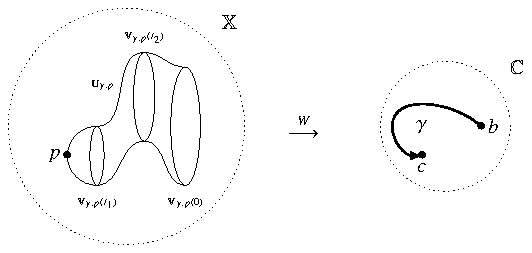
\includegraphics[width=0.66\textwidth]{figures/Fig_080_PDF168_Book156.pdf}
  \caption{消失圈与 Lefschetz thimble（原书 p.156）}
  \label{fig:vanishing-cycle-thimble}
\end{figure}

\begin{example}[二次函数的消失圈]
令 $W\colon\mathbb C^n\to\mathbb C$ 为 $W(z_i)=\sum_i z_i^2$，令 $\gamma\colon[0,1]\to D$ 为 $\gamma(t)=1-t$，并令 $h\colon\mathbb C\to\mathbb R$ 为 $h(z)=\operatorname{Im}z$。写 $z_i=q_i+ip_i$，便有 $hW=\sum_i2p_iq_i$，相应的流方程是
\[
  \dot q_i=-\frac{\partial hW}{\partial p_i}=-2q_i,
  \qquad
  \dot p_i=\frac{\partial hW}{\partial q_i}=2p_i,
\]
其解为 $(q_{0i}e^{-2t},p_{0i}e^{2t})$。流向临界点 $0$ 的点恰好满足 $p_{0i}=0$。因此
\[
  V_{\gamma,0}(t)=\left\{(\vec q,0)\mid\sum_iq_i^2=1-t\right\},
  \qquad
  U_{\gamma,0}=\left\{(\vec q,0)\mid\sum_iq_i^2\le1\right\}.
\]
在 $t=0$ 时，消失圈是超曲面 $\sum_i z_i^2=1$ 中的一个拉格朗日球面，而 thimble 是 $\mathbb C^n$ 中的实球。若换用另一个函数，例如 $h=g\,\operatorname{Im}z$（其中 $g\colon\mathbb C\to\mathbb R$），流方程变为
\[
  \dot q_i=-2q_i\left(g+p_i\frac{\partial gW}{\partial p_i}\right),
  \qquad
  \dot p_i=2p_i\left(g+q_i\frac{\partial gW}{\partial q_i}\right).
\]
方程的精确解会改变，但若 $p_i=0$，它仍保持为零，因此消失圈和 thimble 不变。
\end{example}

\begin{lemma}{消失圈与 Lefschetz thimble 的性质}{vanishing-cycle-exactness}
消失圈与 Lefschetz thimble 分别是 $W^{-1}(\gamma(t))$ 与 $\mathbb C^n$ 中的正合拉格朗日子流形。它们只依赖于 $\gamma$ 和 $W$，而不依赖于 $h$。
\end{lemma}
\begin{proof}[证明梗概]
可以在局部处理这个问题，之后便归结为上面的计算。
\end{proof}

现在假设所有临界值都位于圆盘 $D\subset\mathbb C$ 内，并在圆盘边界上选取基点 $b$。给定从基点到某个临界值的曲线 $\gamma\colon b\to c$ 和临界点 $p\in W^{-1}(c)$，就可以构造消失圈和 thimble。即使流向同一个临界点，不同曲线也会给出不同 thimble。为了研究这些 thimble，我们希望把它们组织成一个范畴。

\begin{definition}{有向 Fukaya 范畴}{directed-fukaya-category}
有向 Fukaya 预范畴 $\mathrm{drFuk}^\bullet(X,W)$ 的对象是所有 Lefschetz thimble $U_{\gamma,p}$，其中 $\gamma\colon[0,1]\to D$ 是从基点 $b$ 到任一临界值 $c=W(p)\in D$ 的曲线，并且 $\gamma$ 在 $b$ 处的切向量指向圆盘内部。给这些 thimble 赋予定向、自旋结构和局部系统。

对象序列 $(U_{\gamma_1,p_1},\ldots,U_{\gamma_k,p_k})$ 称为横截的，若 thimble 两两横截相交，且切向量 $\dot\gamma_1(0),\ldots,\dot\gamma_k(0)$ 的辐角依次递增。换言之，沿基点 $b$ 附近的小圆逆时针行走，进入 $D$ 后会依次遇到 $\gamma_1,\gamma_2$ 等曲线。有向 Fukaya 预范畴的 Hom 空间和乘积按通常方式定义。有向 Fukaya 范畴 $\mathrm{drFuk}^\bullet(X,W)$ 是其范畴化。
\end{definition}
\begin{figure}[H]\centering
  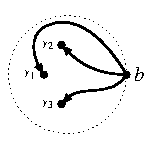
\includegraphics[width=0.26\textwidth]{figures/Fig_081_PDF169_Book157.pdf}
  \caption{基点处有序排列的消失路径（原书 p.157）}
  \label{fig:directed-vanishing-paths}
\end{figure}

\begin{note}\label{note:directed-fukaya-basepoint}
\textbf{注 6.59.} 有向 Fukaya 范畴的定义依赖于边界基点（以及圆盘的大小），但不同选择给出等价范畴，因为可以找到一个旋转边界、但固定临界点的流。这个流会在不同基点对应的有向 Fukaya 范畴之间诱导等价。
\end{note}

\begin{example}[圆环上的 Landau--Ginzburg 模型]\label{ex:punctured-plane-lg-model}
令 $X=\mathbb C^*$，并定义 $W\colon\mathbb C^*\to\mathbb C$，$W(z)=\frac{z-z^{-1}}{4}$。临界点为 $p_\pm=\pm i$，临界值为 $\pm\frac{i}{2}$。取基点 $b=1$，则
\[
  W^{-1}(b)=\left\{x_+,x_-\right\},
  \qquad x_\pm=2\pm\sqrt5.
\]
任取曲线 $\gamma\colon1\to a$，沿 $W$ 提升可得到两条曲线
\[
  \gamma_\pm=2\gamma\pm\sqrt{4\gamma^2+1}.
\]
时刻 $t$ 的消失圈为 $\{\gamma_+(t),\gamma_-(t)\}$，Lefschetz thimble 则是这两条曲线的并。下图展示三个例子和对应的基圆盘路径：
\begin{figure}[H]\centering
  \centering
  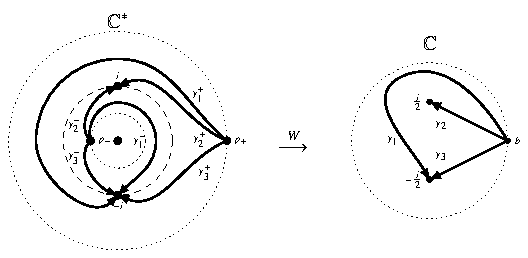
\includegraphics[width=0.74\textwidth]{figures/Fig_082_PDF170_Book158.pdf}\quad
  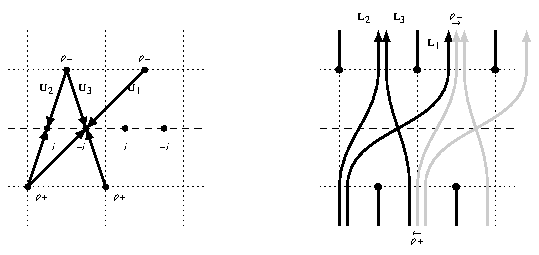
\includegraphics[width=0.53\textwidth]{figures/Fig_083_PDF170_Book158.pdf}
  \caption{圆环上的消失路径及其提升（原书 p.158）}
  \label{fig:punctured-plane-thimbles}
\end{figure}
由于没有浸入圆盘，态射空间为
\[
  \begin{aligned}
  \mathrm{drFuk}^\bullet(U_1,U_2)&=kp_+\oplus kp_-,\\
  \mathrm{drFuk}^\bullet(U_2,U_3)&=kp_+\oplus kp_-,\\
  \mathrm{drFuk}^\bullet(U_1,U_3)&=kp_+\oplus kp_-\oplus kc,
  \end{aligned}
\]
其中 $c$ 表示点 $-i$。

把圆柱展开后，可以看到这一例子与圆的余切丛上、两端各有一个 stop 的 partially wrapped Fukaya 范畴惊人地相似。若在 $p_+$ 与 $p_-$ 附近放置 stop，并把 thimble 两端都延伸到无穷远处，就得到 partially wrapped 范畴中的对象，其态射空间恰好相同。再做一些工作，可以构造函子
\[
  \mathrm{drFuk}^\bullet(\mathbb C^*,W)
  \longrightarrow\mathrm{wrFuk}^\bullet_\sigma(\mathbb C^*),
\]
它在转到导出范畴后成为等价。这一例子说明，在许多情形中，partially wrapped Fukaya 范畴与有向 Fukaya 范畴可以看作同一枚硬币的两面。
\end{example}

\subsection{相对 Fukaya 范畴}\label{subsec:relative-fukaya}
到目前为止所考虑的设定，都是辛流形非紧致的情形。这是因为我们只处理了正合辛流形。

\begin{lemma}{正合辛流形不能紧致}{exact-symplectic-noncompact}
正合辛流形不可能是紧致的。
\end{lemma}
\begin{proof}[证明梗概]
若 $(X,\omega)$ 是 $2n$ 维辛流形，则 $\omega^n$ 是 $X$ 上的体积形式。若 $\omega=d\theta$，则 $\omega$ 的上同调类为零，因而 $\omega^n$ 的上同调类也为零；这不可能，因为体积形式在紧致定向流形上的积分非零。
\end{proof}

为紧致流形定义 Fukaya 范畴颇为困难，因此我们先构造一个中间版本。Seidel 在\bookcite{217}中引入了这一构造。设 $X$ 是紧致 Kähler 流形，且
\[
  D=\bigcup_{i\in I}D_i
\]
是若干光滑、彼此横截相交的复超曲面的并，并假设 $X\setminus D$ 是带柱状端的 Liouville 流形。于是可以按通常方式定义 $X\setminus D$ 上的 Fukaya 范畴。

若把 $D$ 加回去，会发生什么？$\mathrm{exFuk}^\bullet(X\setminus D)$ 中的每个对象也可看成 $X$ 中的拉格朗日膜，且这些对象之间的交点在 $X$ 与 $X\setminus D$ 中相同。但乘积不同：在 $X$ 中可能出现额外的伪全纯圆盘，它们与除子相交，甚至可能有无穷多个。

为了记录这些圆盘，我们考虑由各 $D_i$ 自由生成的幺半群 $G$，并取其形式幂级数环 $k[[G]]$。利用第 3.4.3 节所述技术，应当可以把正合 Fukaya 范畴 $\mathrm{exFuk}^\bullet(X\setminus D)$ 变形为一个带曲率的 $G$-滤过 $A_\infty$ 范畴 $\mathrm{cuFuk}^\bullet(X,D)$，使得对每个
\[
  g=g_1D_1+\cdots+g_kD_k,
\]
都有
\[
  \mu_{k,g}(p_1,\ldots,p_k)=\sum_{p_0}\sum_\psi\sigma_\psi p_0,
\]
其中 $\psi$ 遍历所有与每个 $D_i$ 的交数为 $g_i$ 的全纯映射。要使这一构造成立，还需处理一些问题：
\begin{itemize}
  \item 对每种交数，圆盘的数目都必须有限；
  \item 可能发生圆盘起泡，从而产生 $\mu_0$；
  \item 可能发生球面起泡，球面甚至可能完全包含在某个除子中，因而导致负交数。
\end{itemize}
为解决这些问题，必须限制允许的除子类型，而且可能需要在更大的系数环上工作。更多细节见\bookcite{217,224}。目前，完全一般的构造仍在发展中；不过，概念上的思路如下。

\begin{definition}{相对 Fukaya 范畴}{relative-fukaya-category}
相对 Fukaya 范畴\index{xiangduifukayafanchou@相对 Fukaya 范畴|hyperpage} $\mathrm{cuFuk}^\bullet(X,D)$ 是正合 Fukaya 范畴 $\mathrm{exFuk}^\bullet(X\setminus D)$ 的一个带曲率变形；其乘积按照全纯圆盘与 $D$ 的交型计数。
\end{definition}

\begin{note}\label{note:relative-fukaya-parameter}
\textbf{注 6.63.} 对上述方案的一个重要变体是：不把 $D$ 看成分量 $D_i$ 的并，而是把它视为带自然数系数的线性组合 $D=\sum_i a_iD_i$。这确定一个映射
\[
  k[[G]]\to k[[\hbar]],\qquad
  \hbar^{D_i}\longmapsto\hbar^{a_i},
\]
从而可以把相对 Fukaya 范畴看成定义在 $k[[\hbar]]$ 上的变形，而非定义在 $k[[G]]$ 上。
\end{note}

\begin{note}\label{note:uncurving-relative-fukaya}
\textbf{注 6.64.} 把这个带曲率范畴转化为无曲率范畴有多种方法。最简单的是取带曲率的扭曲复形，并考察满足曲率 $\widehat\mu_0=\lambda1$（其中 $\lambda\in k[[G]]$ 或 $k[[\hbar]]$）的对象所成子范畴。忘掉 $\widehat\mu_0$ 后，这便是一个无曲率滤过范畴，记为 $\lambda\mathrm{Fuk}^{\pm}(X,D)$。若 $X$ 是 Calabi--Yau 流形，可以给 Fukaya 范畴赋予 $\mathbb Z$-分次；此时 $\lambda$ 的次数必须为 $2$，所以只能有 $\lambda=0$。在这种情形下，省略前缀并记作 $\mathrm{Fuk}^\bullet(X,D)$。这些范畴定义在 $k[[G]]$ 上，而 $k[[G]]$ 不是域，因此取极小模型时必须谨慎。

可以沿用第 3.4.3 节的策略，把范畴与 $k((G))$ 作张量，从而得到域上的 $A_\infty$ 范畴并取其极小模型。所得范畴记作
\[
  \lambda D\mathrm{Fuk}^{\pm}(X,D)\otimes k((G))
  \quad\text{或}\quad
  D\mathrm{Fuk}^\bullet(X,D)\otimes k((G)).
\]

有时，$\mathrm{cuFuk}^{\pm}(X,D)$ 中的乘积 $\widehat\mu_k$ 并非形式幂级数，而是实际的多项式。此时，可以通过选取映射 $\rho\colon G\to\mathbb C$，将这些多项式特化为复数。若此外当 $k$ 足够大时 $\widehat\mu_k=0$，就考察满足 $\rho(\widehat\mu_0)=\lambda1$（$\lambda\in\mathbb C$）的扭曲复形；这会给出定义在 $\mathbb C$ 上的无曲率 $A_\infty$ 范畴。
\end{note}

\begin{example}[球面上的相对 Fukaya 范畴]
令 $X$ 为 Riemann 球面，取除子 $D=\{0\}+\{\infty\}$。于是 $X\setminus D=\mathbb C^*=T^*S^1$，系数环取 $k[[\hbar]]$。相对 Fukaya 范畴是
\[
  \mathrm{exFuk}^{\pm}(\mathbb C^*)
  \cong_\infty D\mathrm{mod}^{\pm}\mathbb C[X,X^{-1}]
\]
的一个变形。注意，这只能是 $\mathbb Z_2$-分次变形，因为体积形式 $dz/z$ 不能延拓到 Riemann 球面。

若 $(L,\rho_M)$ 是底圆，且局部系统的平行移动由 $M\in\mathbb C^*$ 给出，那么有两个以 $S^1$ 为边界的全纯圆盘：球面的上半部和下半部。它们分别穿过 $0$ 与 $\infty$；边界定向相反，因此沿圆的平行移动互为逆。把所有 $\mu_0$ 乘积合起来，得到
\[
  \widehat\mu_0\big|_{(L,\rho_M)}
  =(M\hbar+M^{-1}\hbar)\,\iota.
\]
\begin{figure}[H]\centering
  \centering
  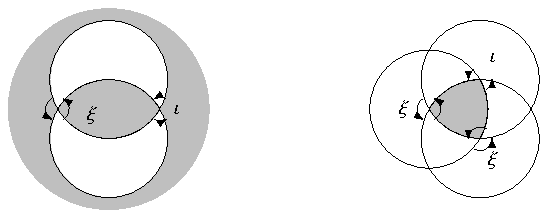
\includegraphics[width=0.73\textwidth]{figures/Fig_084_PDF173_Book161.pdf}
  \caption{穿过除子两分支的圆盘（原书 p.161）}
  \label{fig:relative-fukaya-sphere-disks}
\end{figure}

为了确定 $(L,\rho_M)$ 的自同态之间的乘积，我们考察一列与圆同痕的拉格朗日子流形。对一元乘积有两个圆盘贡献；其他乘积各只有一个贡献，因为另一个圆盘会多次绕过 $\infty$，不再是浸入。于是
\[
  \widehat\mu_1(\xi)=(M\hbar-M^{-1}\hbar)\,\iota,
  \qquad
  \widehat\mu_k(\xi,\ldots,\xi)=M\hbar\,\iota\quad(k\ge2).
\]
因此，除非 $M=\pm1$，对象 $(L,\rho_M)$ 都是零对象。把剩下两个对象记为 $L_\pm$。它们是曲率分别为 $\pm2\hbar$ 的带曲率对象，但可以视为无曲率范畴
$\pm2\hbar\,\mathrm{Fuk}^{\pm}(X,D)\otimes k((\hbar))$ 中的对象。经过一次 $A_\infty$ 同构，可以令 $\widehat\mu_{\ge3}=0$，因此这两个对象的自同态环为
\[
  \frac{k((\hbar))[\xi]}{(\xi^2\pm\hbar)}.
\]
\end{example}

\subsection{完整 Fukaya 范畴}\label{subsec:full-fukaya}
我们已经走到旅程的最后阶段：完整 Fukaya 范畴。给定紧致 Kähler 流形 $(X,\omega,J)$，该范畴应纳入所有拉格朗日膜。如前所述，非正合性意味着圆盘的辛面积没有上界，因此不能直接应用 Gromov 紧致性定理来证明给定一组拉格朗日子流形边界时全纯多边形只有有限多个。因此，乘积可能包含无穷多项，甚至未必定义良好。

尽管如此，对任意给定上界，面积低于该上界的全纯多边形仍然只有有限多个。因此，一般而言，乘积会是按面积递增排列的项所组成的级数。于是可以在滤过设定下工作。令 $G\subset\mathbb R_{\ge0}$ 为所有可能出现的全纯圆盘面积生成的幺半群。环 $k[[G]]$ 可视为 Novikov 域\index{novikovyu@Novikov 域|hyperpage}的子环；Novikov 域由实指数递增的幂级数构成：
\[
  V=\left\{\sum_{i=0}^{\infty}\lambda_iT^{r_i}\ \middle|\ 
  \lambda_i\in k,\ r_i\in\mathbb R,\ i>j\Rightarrow r_i>r_j\right\}.
\]

要从这里得到定义良好的范畴仍很技术性，并且需要限制允许的流形类型（例如无环流形，或满足 $\langle\pi_2(X),\omega\rangle=0$ 的流形）和膜类型（例如单调膜）。考虑这些限制后，便得到完整 Fukaya 范畴。其构造和技术细节超出本书范围，更多信息可参阅专著\bookcite{83,84}。

在理想情形下，我们得到一个 $G$-滤过的带曲率 $A_\infty$ 范畴 $\mathrm{cuFuk}^{\pm}_V(X)$，其对象是带有 $U_n$-局部系统的紧致拉格朗日膜。对任意 $\lambda\in V$，曲率为 $\lambda$ 的带曲率扭曲对象构成 Novikov 域上的普通 $A_\infty$ 范畴 $\lambda\mathrm{Fuk}^{\pm}_V(X)$。

\begin{note}\label{note:unitary-local-systems}
\textbf{注 6.66.} 这里只使用 $U_n$-局部系统，而不使用 $\mathrm{GL}_n$-局部系统，是因为局部系统的实部可以吸收到拉格朗日子流形的位置中。例如，对 $T^*S^1=\mathbb C^*$，带有实局部系统的底圆 $\{|z|=1\}$ 可解释为移位后的圆 $\{|z|=r\}$ 配上平凡局部系统。注意，后者不是正合拉格朗日子流形，因此不属于 $\mathrm{exFuk}^\bullet(\mathbb C^*)$，但它是完整 Fukaya 范畴 $\mathrm{Fuk}^\bullet_V(\mathbb C^*)$ 的对象。
\end{note}

\begin{example}[环面上的 theta 函数]
令 $T=\mathbb C/(\mathbb Z+i\mathbb Z)$ 为带标准辛结构的环面，坐标为 $z=q+ip$，辛形式为 $\omega=a\,dp\wedge dq$。考察 Fukaya 范畴中的三个对象 $L_0,L_1,L_2$，分别对应方程
\[
  q=0,\qquad p=0,\qquad p+q=\frac12.
\]
三个交点为
\[
  p_1=(0,0)\in L_0\cap L_1,\quad
  p_2=(\tfrac12,0)\in L_1\cap L_2,\quad
  p_0=(0,\tfrac12)\in L_0\cap L_2.
\]
为了求乘积 $\mu(p_2,p_1)$，要统计以 $p_0,p_1,p_2$ 为角点的浸入三角形。在万有覆盖上，这些三角形都是等腰直角三角形。固定 $p_1$ 后，三角形由一条边的长度及其定向唯一确定；边长是奇数个半单位，即 $(2k+1)/2$，相应面积为 $\frac a8(2k+1)^2$。所得幂级数可以用 Jacobi theta 函数 $\vartheta_2(z,t)$ 整齐地表示：
\begin{figure}[H]\centering
  \centering
  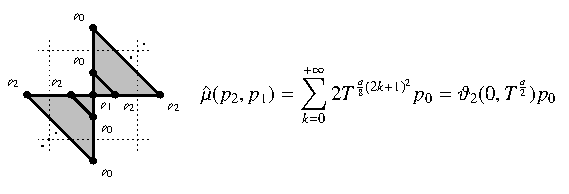
\includegraphics[width=0.72\textwidth]{figures/Fig_085_PDF174_Book162.pdf}
  \caption{环面上三角形的计数与 theta 函数（原书 p.162）}
  \label{fig:torus-triangles-theta}
\end{figure}
\[
  \widehat\mu(p_2,p_1)=
  \sum_{k=0}^{+\infty}2T^{\frac a8(2k+1)^2}p_0
  =\vartheta_2(0,T^{a/2})p_0.
\]
\end{example}

\subsection{联系}\label{subsec:fukaya-connections}
设 $(X,\omega,J)$ 是 Kähler 流形，$D$ 是使得 $\breve X:=X\setminus D$ 成为 Liouville 流形的除子，并设 $W\colon\breve X\to\mathbb C$ 是全纯函数。在理想情形下，可以找到一组 stop $\sigma$，阻断 thimble 锥形端不同部分之间的所有 Reeb 弦。此时会得到如下 $A_\infty$ 范畴关系图：
\begin{figure}[H]\centering
  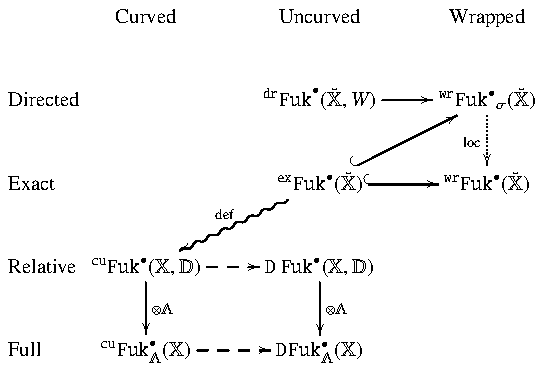
\includegraphics[width=0.86\textwidth]{figures/Fig_086_PDF175_Book163.pdf}
  \caption{$A_\infty$ 范畴之间的联系（原书 p.163）}
  \label{fig:fukaya-category-connections}
\end{figure}
蛇形箭头表示变形，点线箭头表示局部化，虚线箭头表示取无曲率扭曲复形。指向最下行的箭头表示先改变底环，再作嵌入。

\section{生成元}\label{sec:fukaya-generators}
前面已经看到，定义 Fukaya 范畴时有许多不同选择：可以纳入或排除不同类型的对象，也可以允许或禁止某些态射。这些选择会产生彼此相关但并不相同的范畴。转向导出范畴或分裂导出范畴，可以解决其中一部分问题；从表示论的角度看，这样便把本应属于范畴的对象都纳入进来。

这种做法往往也使范畴更容易描述：我们可以寻找一组生成元，并尝试把整个范畴看成少数对象的扭曲完备化。相比整个范畴，此时只需描述这些对象之间的部分或全部态射乘积，便能相当细致地刻画分裂导出 Fukaya 范畴。

\takeaway{次数为 $1$ 的态射 $x\colon L_1\to L_2$ 给出拉格朗日手术 $L_1+_xL_2\cong\operatorname{Cone}(x)$，这是用锥判定生成的基本手段；由此可知余切丛由单个余切纤维生成、曲面上的弧系生成 wrapped Fukaya 范畴，Abouzaid 判据则用开闭映射检测生成性。}

\subsection{Fukaya 范畴中的锥}\label{subsec:fukaya-cones}
要理解几何上何谓生成 Fukaya 范畴，先要考察锥构造。设两个拉格朗日子流形 $L_1,L_2$ 在一点 $x$ 横截相交。在 $x$ 的邻域内可取典范坐标 $p_i,q_i$，使得 $L_1$ 由方程 $p_i=0$ 给出，$L_2$ 由方程 $q_i=0$ 给出。

\begin{figure}[H]\centering
  \centering
  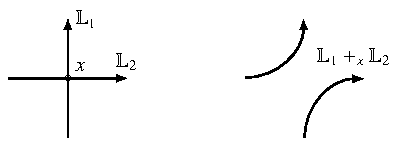
\includegraphics[width=0.72\textwidth]{figures/Fig_087_PDF176_Book164.pdf}
  \caption{横截交点处的拉格朗日手术（原书 p.164）}
  \label{fig:lagrangian-surgery-cone}
\end{figure}

对任意 $\varepsilon>0$，由方程 $p_iq_i+\varepsilon=0$ 定义的子流形 $L_\varepsilon$ 是拉格朗日子流形；不同 $\varepsilon$ 对应的子流形之间存在 Hamilton 同伦，其生成函数在 $L_\varepsilon$ 邻域内为 $f=\sum_i\log(p_iq_i)$。我们可以构造一个拉格朗日子流形 $L_1+_xL_2$：它在 $x$ 附近的开球内与 $L_\varepsilon$ 相同，在稍大的开球之外与 $L_1\cup L_2$ 相同；在两个球之间稍作调整，使两部分平滑接合。对任意交点 $x$ 都可以这样做；不过，若要使定向相容，还需要交点 $x$ 的 $\mathbb Z_2$ 次数为 $1$。

\begin{theorem}{拉格朗日手术与锥}{lagrangian-surgery-is-cone}
对象 $L_1+_xL_2$ 同构于 $\operatorname{Cone}(x)$，其中 $x$ 被视为次数为 $1$ 的态射 $x\colon L_1\to L_2$。
\end{theorem}
\begin{proof}[证明思路]
取任意一个与 $L_1+_xL_2$ 横截相交、且不进入我们作粘接的 $x$ 邻域开球的拉格朗日子流形 $U$。由于每个交点都落在 $L_1$ 或 $L_2$ 上，Floer 复形分解为
\[
  CF(L_1+_xL_2,U)=CF(L_1,U)\oplus CF(L_2,U).
\]
若有一个全纯 $n$ 边形，其一条边界落在 $L_1+_xL_2$ 上，就令 $\varepsilon\to0$ 对它作退化。所得全纯圆盘的边界落在 $L_1\cup L_2$ 上，可能完全位于 $L_1$ 上、完全位于 $L_2$ 上，或同时经过二者。前两种情形下，$n$ 边形仍是 $n$ 边形；第三种情形下，它变成一个多出角点 $x$ 的 $(n+1)$ 边形。因此，凡是含有 $L_1+_xL_2$ 的 $(n-1)$ 元乘积，都等于通常的 $(n-1)$ 元乘积与插入一个额外 $x$ 的 $n$ 元乘积之和。这正是锥构造中的乘积规则。
\end{proof}

\begin{note}\label{note:cone-multiple-intersections}
\textbf{注 6.69.} 若 $L_1$ 与 $L_2$ 有多个交点，那么 $L_1+_xL_2$ 通常不是嵌入的拉格朗日子流形，而是一个浸入。另一种可能是 $L_1+_xL_2$ 由多个连通分支组成；此时应把每个分支看作 $\operatorname{Cone}(x)$ 的一个直和项。
\end{note}

\begin{note}\label{note:cone-extensions}
\textbf{注 6.70.} 这个构造有若干推广。
\begin{itemize}
  \item 若 $L_1,L_2$ 带有局部系统，且态射为 $\alpha x$，其中 $\alpha\colon L_1(x)\to L_2(x)$ 是可逆线性映射，则可以在 $L_1+_xL_2$ 上定义新的局部系统。先在 $L_1+_xL_2$ 的每个连通分支上选取一个基点，要求在退化到 $L_1\cup L_2$ 时该基点不趋于 $x$。基点处的每条闭路在退化后成为 $L_1\cup L_2$ 上的一条折线路径，其各段分别落在 $L_1$ 或 $L_2$ 上，并在 $x$ 处衔接。沿各段使用原有局部系统的线性映射；每次从 $L_1$ 转到 $L_2$ 时插入 $\alpha$，反向转接时插入 $\alpha^{-1}$，便得到所需的整体映射。
  \item 若 $L_1,L_2$ 在多个点 $x_1,\ldots,x_k$ 相交，则可把 $\alpha_1x_1+\cdots+\alpha_kx_k$ 的锥理解为同时在这些交点处作手术得到的新拉格朗日子流形。
\end{itemize}
\end{note}

\subsection{余切丛的生成元}\label{subsec:cotangent-generators}
考察圆柱 $X=T^*S^1=\mathbb C^*$，并赋予它标准体积形式 $dz$。我们曾得到如下包含链：
\[
  \mathrm{Fuk}^{\mathrm{ba}}X\subset \mathrm{Fuk}^{\mathrm{ex}}X\subset \mathrm{Fuk}^{\mathrm{wr}}X.
\]
第一个范畴在移位意义下只有一个对象 $L_1$，其自同态环为 $k[\xi]/(\xi^2)$。在第二个范畴中，每个不可分解对象在移位意义下都对应一个圆及其上的局部系统 $\rho$。第三个范畴还包含非紧拉格朗日子流形，例如余切纤维 $U=T_x^*S^1$。

余切纤维的自同态环为 $k[X,X^{-1}]\cong k[\pi_1(S^1)]$，并且它生成 $\mathrm{Fuk}^{\mathrm{wr}}X$。事实上，任意非紧拉格朗日子流形都同构于 $U$ 的某个移位。若 $L$ 是带有局部系统 $\rho\colon\pi_1(S^1)\to\mathrm{GL}_n$ 的圆，则可将 $L$ 识别为 $\operatorname{Cone}(f)$，其中 $f=(1+\rho(\ell))1_n$ 是从 $U^{\oplus n}$ 到 $U[-1]^{\oplus n}$ 的次数 $1$ 态射，$\ell$ 是圆周基本群的生成元。

几何上，取 $1+\rho(\ell)X$ 的锥，会在两点处把 $\phi_1^h(U)$ 与 $U$ 粘接起来，得到三条曲线：一条闭曲线和圆柱两端各一条开曲线。后两条是零对象；闭曲线则是带有局部系统的紧致拉格朗日子流形。沿圆周的平行移动恰为 $\rho(\ell)$，因为在一处用恒等矩阵粘接纤维，在另一处则用 $\rho(\ell)$ 粘接。

\begin{figure}[H]\centering
  \centering
  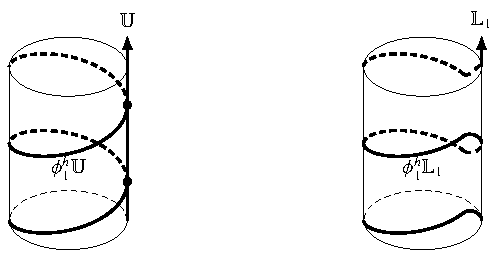
\includegraphics[width=0.76\textwidth]{figures/Fig_088_PDF178_Book166.pdf}
  \caption{圆柱上由余切纤维构造锥（原书 p.166）}
  \label{fig:cylinder-cotangent-cone}
\end{figure}

对于正合 Fukaya 范畴，情形有所不同。由于其中没有这些非紧对象，不存在有限生成集。要生成所有可能的局部系统，就需要对 $\rho(\ell)$ 的每个可能特征值各取一个生成元。因此，分裂导出正合 Fukaya 范畴由所有 $L_\lambda$ 生成，其中 $L_\lambda$ 是带一维局部系统、且 $\rho(\ell)=\lambda$ 的圆。它们之中只有 $L_1$ 属于基本 Fukaya 范畴，并生成该范畴：
\[
  D^\pi\mathrm{Fuk}^{\mathrm{ba}}X\simeq\langle L_1\rangle
  \subset D^\pi\mathrm{Fuk}^{\mathrm{ex}}X=\langle L_\lambda\mid\lambda\in k^*\rangle
  \subset D^\pi\mathrm{Fuk}^{\mathrm{wr}}X=\langle U\rangle.
\]
Abouzaid 对圆柱上 wrapped Fukaya 范畴的生成结论可以推广到所有余切丛；详细论证见文献\bookcite{7}。

\begin{theorem}{Abouzaid 生成定理}{abouzaid-cotangent-generation}
设 $M$ 是紧致连通黎曼流形。余切丛 $X=T^*M$ 的 wrapped Fukaya 范畴由一个余切纤维生成：
\[
  D^\pi\mathrm{Fuk}^{\mathrm{wr}}T^*M=\langle T_x^*M\rangle.
\]
\end{theorem}
\begin{proof}[证明思路]
首先，所有余切纤维彼此同构。由 $x$ 到 $y$ 的测地线给出 $T_x^*M$ 与 $T_y^*M$ 之间的一条 Reeb 弦；它是可逆态射，因为其逆对应于沿同一测地线反向行进。

现在取一个与零截面 $M$ 横截相交的拉格朗日子流形 $L$。选取函数 $f\colon M\to\mathbb R$，使其零点恰为交点，并考察流像 $\phi_f^tL$。当 $t\to\infty$ 时，这个流像趋于位于这些交点处的余切纤维之并。因此，$\phi_f^tL$ 可以看成这些余切纤维之间某个态射的锥。具体而言，该态射是若干 Reeb 弦之和；相对于余切纤维，这些 Reeb 弦同伦于连接交点的曲线。

\begin{figure}[H]\centering
  \centering
  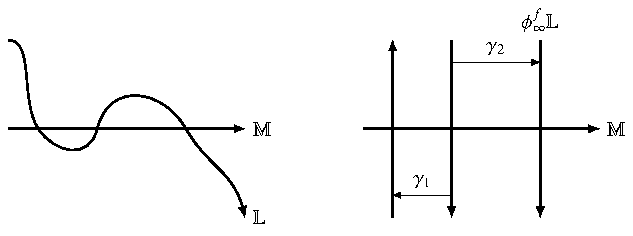
\includegraphics[width=0.76\textwidth]{figures/Fig_089_PDF179_Book167.pdf}
  \caption{拉格朗日子流形流向余切纤维之并（原书 p.167）}
  \label{fig:cotangent-flow-limit}
\end{figure}
\end{proof}

\begin{corollary}{Abouzaid}{abouzaid-loop-space}
余切丛的 wrapped Fukaya 范畴与环路空间上同调环的导出范畴分裂导出等价：
\[
  D^\pi\mathrm{Fuk}^{\mathrm{wr}}T^*M\simeq D^\pi H^\bullet(\mathcal L_xM).
\]
\end{corollary}
\begin{proof}[证明思路]\par
从 $T_x^*M$ 到自身的 Reeb 弦构成环路空间上某个 Morse 函数的临界点。因此，$\mathrm{Fuk}^{\mathrm{wr}}(T_x^*M,\allowbreak T_x^*M)$ 可以解释为环路空间上同调的一种模型。
\end{proof}

\subsection{有向 Fukaya 范畴的生成元}\label{subsec:directed-generators}
对于有向 Fukaya 范畴，可以构造许多生成集。设 $W\colon X\to\mathbb C$ 是 Lefschetz 纤维化，有 $k$ 个不同临界点 $p_i$，对应临界值 $c_i=W(p_i)$，且这些临界值彼此不同。选取 $k$ 条曲线 $\gamma_i$，使每条曲线都从基点 $b$ 出发，分别通向一个临界值；再假设这些曲线从 $b$ 出发的方向互不相同，且仅在 $b$ 相交。这样的曲线系称为一个例外序列\index{liewaixulie@例外序列|hyperpage}。

\begin{theorem}{Seidel 生成定理}{seidel-directed-generation}
例外序列对应的 thimble 生成有向 Fukaya 范畴：
\[
  D^\pi\mathrm{Fuk}^{\mathrm{dr}}(X,W)=\langle U_{\gamma_i}\mid i=1,\ldots,k\rangle.
\]
\end{theorem}
\begin{proof}[证明思路]
每条从 $b$ 到某临界值的互不相交曲线都可以扩充为一个例外序列。可以证明，任意两个例外序列都能通过称为变异的过程互相转换：取基点处相邻的两条曲线，在其中一条上添加绕另一条一周的环路，从而交换它们的次序。

可以证明，变异后新得到的 thimble 可由原 thimble 取锥表示，反过来也成立。因此，两组 thimble 生成同一个范畴。由于每个 thimble 都能出现在某个例外序列中，每个例外序列都生成全部 thimble。
\end{proof}

\begin{example}[圆柱上的 Lefschetz 纤维化]\label{ex:lefschetz-cylinder-quiver}
例~\ref{ex:punctured-plane-lg-model} 中考察了 Lefschetz 纤维化 $\pi\colon\mathbb C^*\to\mathbb C$，$z\mapsto\frac{z-z^{-1}}{4}$。它有两个临界点，临界值为 $\pm\frac{i}{2}$。我们考虑了三条曲线 $\gamma_1,\gamma_2,\gamma_3$；其中 $\gamma_1,\gamma_2$ 构成一个例外序列，$\gamma_2,\gamma_3$ 也构成一个例外序列。前者是后者的一次变异。两种情况下，自同态环都是二顶点双箭图的路径代数。因此
\begin{figure}[H]\centering
  \centering
  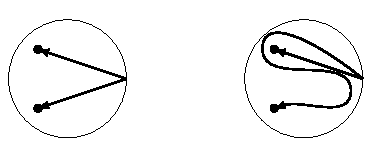
\includegraphics[width=0.48\textwidth]{figures/Fig_090_PDF180_Book168.pdf}
  \caption{例外序列的变异（原书 p.168）}
  \label{fig:mutation-two-curves}
\end{figure}
\begin{figure}[H]\centering
  \centering
  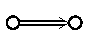
\includegraphics[width=0.36\textwidth]{figures/Fig_091_PDF180_Book168.pdf}
  \caption{二顶点双箭图（原书 p.168）}
  \label{fig:two-vertex-quiver-example}
\end{figure}
\[
  D^\pi\mathrm{Fuk}^{\mathrm{dr}}(\mathbb C^*,W)
  \cong_\infty D^\pi\mathrm{mod}^{\bullet}(Q),\qquad
  Q=\left(\bullet\rightrightarrows\bullet\right).
\]
\begin{figure}[H]\centering
  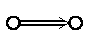
\includegraphics[width=0.34\textwidth]{figures/Fig_092_PDF180_Book168.pdf}
  \caption{该例中的二顶点箭图（原书 p.168）}
\end{figure}
\end{example}

\begin{example}[五次多项式的 thimble]\label{ex:quintic-thimbles}
令 $W\colon\mathbb C\to\mathbb C$，$Z\mapsto \frac45Z^5+Z$。其临界点为 $\frac{\pm1\pm i}{2}$，临界值为 $\frac{2(\pm1\pm i)}{5}$。基点 $1\in\mathbb C$ 上方的纤维由五个点组成。下图画出六条曲线 $\gamma_i$，它们从基点连向这些临界值。每条曲线对应一个 thimble $U_i$ 和一个消失圈 $V_i$；消失圈是两个点组成的集合，thimble 则是连接这两点的线段。

\begin{figure}[H]\centering
  \centering
  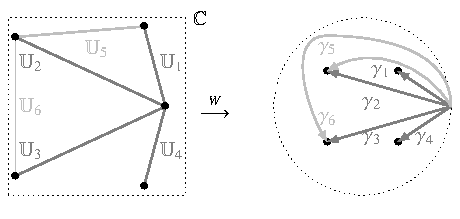
\includegraphics[width=0.84\textwidth]{figures/Fig_093_PDF180_Book168.pdf}
  \caption{五次多项式的临界值、thimble 与消失圈（原书 p.168）}
  \label{fig:quintic-thimbles}
\end{figure}

四元组 $\gamma_1,\ldots,\gamma_4$ 构成一个例外序列。在这个例子中，所有消失圈都包含同一个点，因此每对顶点之间都有态射。进一步考察可知，消失圈的自同态环是下列线性箭图的路径代数：
\begin{figure}[H]\centering
  \centering
  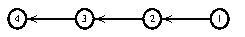
\includegraphics[width=0.43\textwidth]{figures/Fig_094_PDF180_Book168.pdf}
  \caption{例外序列对应的线性箭图（原书 p.168）}
  \label{fig:linear-quiver-exceptional-sequence}
\end{figure}
\[
  Q=\left(4\longleftarrow3\longleftarrow2\longleftarrow1\right).
\]

若将 $\gamma_2$ 绕 $\gamma_1$ 变异，便得到 $\gamma_5$；若先将 $\gamma_3$ 绕 $\gamma_2$ 变异，再绕 $\gamma_1$ 变异，也会得到 $\gamma_6$。
% [Tutor Note: 原书 p.169 此处两处均作“变成 $\gamma_5$”，但同段随即写“以 $\gamma_5,\gamma_6$ 替换 $\gamma_2,\gamma_3$”，且下一句按 $\gamma_6,\gamma_5$ 计顶点次序；第二次变异（先绕 $\gamma_2$、再绕 $\gamma_1$）应为 $\gamma_6$。译文径改，对照原书时请注意。]

以 $\gamma_5,\gamma_6$ 替换 $\gamma_2,\gamma_3$ 后，顶点次序发生交换，因为 $\gamma_6,\gamma_5$ 的起始角度小于 $\gamma_1$。此时只有相邻的消失圈相交，故自同态环成为对偶箭图代数（其中所有箭头乘积均为零）：
\begin{figure}[H]\centering
  \centering
  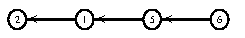
\includegraphics[width=0.43\textwidth]{figures/Fig_095_PDF181_Book169.pdf}
  \caption{变异后得到的线性箭图（原书 p.169）}
  \label{fig:mutated-linear-quiver}
\end{figure}
此时的箭图依次连接顶点 $2,1,5,6$，且相邻箭头的乘积均为零。
这两个代数都生成线性箭图的导出范畴。
\end{example}

\subsection{生成判据}\label{subsec:generation-criteria}
一般而言，判断一组拉格朗日膜是否分裂生成 Fukaya 范畴并不容易。锥的几何解释提示我们：要寻找分裂生成元，应当找到一组拉格朗日子流形，使每个拉格朗日子流形都能经 Hamilton 同伦变形到由这组子流形拼成的极限。

\begin{example}[曲面上的弧]
若 $X$ 是曲面，可以令这些拉格朗日子流形把曲面切分为拓扑平凡的区域，例如多边形或条带。比如，取一个带有标记点 $m_1,\ldots,m_k$ 的紧致黎曼曲面 $\Sigma$。删去标记点所得的曲面 $\Sigma^\times=\Sigma\setminus\{m_1,\ldots,m_k\}$，可通过在每个标记点附近挖去小圆盘并粘上无限圆柱，而获得 Liouville 流形结构。对连接两个标记点的每条曲线，我们在 $\mathrm{Fuk}^{\mathrm{wr}}\Sigma^\times$ 中得到一个非紧拉格朗日子流形，称为一条弧。下面给出了一个由四条弧分成两个正方形的双穿孔环面。

\begin{figure}[H]\centering
  \centering
  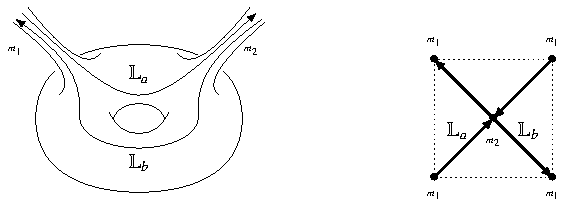
\includegraphics[width=0.77\textwidth]{figures/Fig_096_PDF181_Book169.pdf}
  \caption{弧将双穿孔环面分为两个正方形（原书 p.169）}
  \label{fig:arcs-two-punctured-torus}
\end{figure}

每条弧都可看作 wrapped Fukaya 范畴中的对象；弧之间的 Reeb 弦对应标记点周围的逆时针角。一个角的锥会把两条弧粘成一条新弧。也可以用多个角之和的锥粘接两条以上的弧，从而得到带局部系统的闭曲线。
\end{example}

\begin{theorem}{曲面上弧的生成判据}{arcs-generate-surface-fukaya}
若一组弧把曲面 $\Sigma$ 切分为多边形，则这组弧生成 wrapped Fukaya 范畴 $D^\pi\mathrm{Fuk}^{\mathrm{wr}}\Sigma^\times$。
\end{theorem}
\begin{proof}[证明思路]
若这些弧将曲面切分为多边形，就可以用沿着曲线所经过的多边形边界行进的弧序列来逼近任意曲线。因此，借助锥构造，可以得到任意曲线。

\begin{figure}[H]\centering
  \centering
  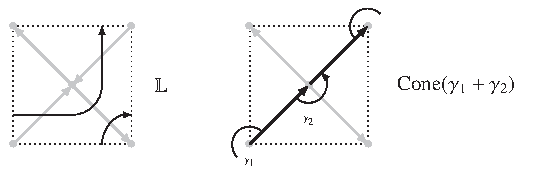
\includegraphics[width=0.72\textwidth]{figures/Fig_097_PDF182_Book170.pdf}
  \caption{通过角的锥拼接弧（原书 p.170）}
  \label{fig:cone-of-angles-arcs}
\end{figure}
\end{proof}

\begin{note}\label{note:surface-arcs-combinatorial}
\textbf{注 6.78.} 用弧生成曲面 Fukaya 范畴的思想将在本书第三部分进一步展开。它使我们能够组合地定义 Fukaya 范畴，并避开辛几何中大多数技术细节。
\end{note}

对于高维辛流形，情形更为复杂，因为拉格朗日膜并不会把流形切分为互不相交的区域。Abouzaid \bookcite{6} 给出了另一种检验一组拉格朗日膜是否生成 wrapped Fukaya 范畴的方法。其基本思想是：要成为分裂生成元，膜之间的态射必须充分反映 Reeb 流。为测量这一点，我们需要比较两个复形。

\begin{definition}{Hochschild 同调}{hochchild-homology-generators}
设 $\{L_i\}_{i\in I}$ 是一组拉格朗日膜，$L$ 是它们在 Fukaya 范畴中直和 $\bigoplus_iL_i$ 的自同态代数。Hochschild 同调\index{hochschildtongdiao@Hochschild 同调|hyperpage} $HH_\bullet(L)$ 定义为复形
\[
  CC_\bullet:=\bigoplus_{k=0}^{\infty}L\otimes L[1]^{\otimes k}
\]
的同调，其中微分由各个 $A_\infty$ 乘积给出：
\[
\begin{aligned}
 d(\gamma_0\otimes\cdots\otimes\gamma_k)
 ={}&\sum_{i>j}\pm\mu(\gamma_i,\ldots,\gamma_k,\ldots,\gamma_j)
       \otimes\gamma_{j+1}\otimes\cdots\otimes\gamma_{i-1}\\
 &+\sum_{i<j}\pm\gamma_0\otimes\cdots\otimes\gamma_i
       \otimes\mu(\gamma_{i+1},\ldots,\gamma_j)
       \otimes\gamma_{j+1}\otimes\cdots\otimes\gamma_k.
\end{aligned}
\]
% [Tutor Note: 这里已把第一个和式中的指标改为 $\gamma_{j+1}\otimes\cdots\otimes\gamma_{i-1}$：当 $\mu$ 作用于循环区间 $\gamma_i,\ldots,\gamma_k,\gamma_0,\ldots,\gamma_j$ 时，余下恰是 $\gamma_{j+1},\ldots,\gamma_{i-1}$；原文 p.170 印作 $\gamma_{i+j+1}$，疑为笔误。另外 Hochschild 同调在此记作 $HH_\bullet$，与 $CC_\bullet$ 的下标一致。]
\end{definition}

\begin{note}\label{note:hochchild-general}
\textbf{注 6.80.} Hochschild 同调是代数对象，对任意 $A_\infty$ 代数或范畴都可以定义\bookcite{253,93}。对多项式环 $\mathbb C[X_1,\ldots,X_n]$，它同构于多项式微分形式环
\[
  \mathbb C[X_1,\ldots,X_n]\langle dX_1,\ldots,dX_n\rangle.
\]
这称为 Hochschild--Kostant--Rosenberg 定理\bookcite{160,253}，并且对所有光滑仿射簇的坐标环都成立（见第\ref{ch:algebraic-geometry}章）。
\end{note}

\begin{definition}{辛同调}{symplectic-homology-generation}
设 $(X,\theta)$ 是带柱形端的 Liouville 流形。辛同调\index{xintongdiao@辛同调|hyperpage}是复形 $SC^\bullet(X)$ 的同调。该复形由某个适当通有的含时 Hamilton 函数所对应的 Reeb 流轨道生成，微分通过计数伪全纯圆柱定义：
\[
  d\rho_1=\sum_{\rho_2}\sum_{\psi\in\mathcal M(\rho_1,\rho_2)}\sigma_\psi\,\rho_2,
\]
其中 $\mathcal M(\rho_1,\rho_2)$ 表示连接 $\rho_1$ 与 $\rho_2$ 的刚性伪全纯圆柱模空间，$\sigma_\psi$ 是相应的符号。
\begin{figure}[H]\centering
  \centering
  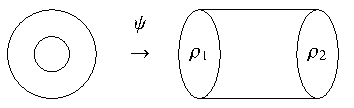
\includegraphics[width=0.48\textwidth]{figures/Fig_098_PDF183_Book171.pdf}
  \caption{辛同调微分所计数的伪全纯圆柱（原书 p.171）}
  \label{fig:symplectic-homology-cylinder}
\end{figure}
\end{definition}

\begin{note}\label{note:symplectic-homology-ainfty}
\textbf{注 6.82.} 辛同调带有 $A_\infty$ 结构，该结构通过计数从单位圆盘出发、挖去若干小圆盘的全纯映射得到；在此结构下，它还具有一个同伦意义下的单位元。关于辛同调的更多内容，见文献\bookcite{53,78,255,182}。
\end{note}

\begin{definition}{开闭映射}{open-closed-map}
开闭映射\index{kaibiyingshe@开闭映射|hyperpage} $OC\colon CC_\bullet(L)\to SC^\bullet(X)$ 通过计数以 Reeb 弦为角点、以 Reeb 轨道为另一端的带符号全纯映射 $\psi$ 定义：
\[
  OC(\gamma_1\otimes\cdots\otimes\gamma_k)=\sum_{\rho}\sum_{\psi\in\mathcal M(\gamma_1,\ldots,\gamma_k;\rho)}\sigma_\psi\,\rho.
\]
这里 $\mathcal M(\gamma_1,\ldots,\gamma_k;\rho)$ 是具有指定 Reeb 弦角点及 Reeb 轨道端的全纯映射模空间，$\sigma_\psi$ 表示其符号。
\begin{figure}[H]\centering
  \centering
  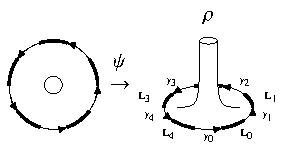
\includegraphics[width=0.62\textwidth]{figures/Fig_099_PDF183_Book171.pdf}
  \caption{开闭映射所计数的全纯曲面（原书 p.171）}
  \label{fig:open-closed-map}
\end{figure}
该映射是复形间的态射，因而在同调上诱导映射
\[
  OC\colon HH_\bullet(L)\longrightarrow SH^\bullet(X).
\]
% [Tutor Note: 开闭映射是链映射并不显然：需把“一端为 Reeb 轨道、另一端为若干 Reeb 弦”的圆柱模空间紧化，使其边界项分别对应 Hochschild 微分与辛同调微分；为此要对含时 Hamilton 函数取一般位置，否则会出现伪全纯圆柱的破裂。原文把验证留给文献 6。]
\end{definition}

\begin{theorem}{Abouzaid 生成判据}{abouzaid-generation-criterion}
若单位元 $1\in SH^\bullet(X)$ 属于 $OC$ 的像，则 $\{L_i\}_{i\in I}$ 分裂生成 $X$ 的 wrapped Fukaya 范畴。
\end{theorem}
\begin{proof}[证明思路]
给定任意拉格朗日膜 $B$，由该判据可找到一组高阶乘积，使得
\[
  1_B=\sum_r\mu(\gamma_{r,1},\ldots,\gamma_{r,k_r}).
\]
引理\ref{lem:split-generation-criterion} 随即说明 $B$ 由 $L$ 分裂生成。
\end{proof}

\begin{example}[圆柱上的 Abouzaid 判据]
Abouzaid 判据最基本的例子\bookcite{6} 是 $X=T^*S^1$。此时余切纤维 $T_x^*M$ 是生成元。$L=\mathbb C[X^{\pm1}]$ 的 Hochschild 同调为微分形式环 $\mathbb C[X^{\pm1}]\langle dX\rangle$，其中 $dX$ 简记为 $1\otimes X-X\otimes1$。

在辛同调中，绕圆柱 $i$ 圈的每个 Reeb 轨道 $\gamma_i$ 给出两个元素 $\gamma_i[0],\gamma_i[1]$，其次数分别为 $0$ 和 $1$。（若 Hamilton 函数与时间无关，闭 Reeb 轨道会产生一圈起点各异的 Reeb 轨道；对 Hamilton 函数作扰动后，这个圆周对称性破缺，只留下两个轨道。）当 $i=0$ 时，这两个元素对应于流为零处的“常值环路”。所以每个次数和同调类恰好各有一个基元素。开闭映射保持这两种分次，并给出同构，将 $X^i$ 映到 $\gamma_i[0]$，将 $X^idX$ 映到 $\gamma_i[1]$。
\end{example}

\begin{note}\label{note:compact-generation-criterion}
\textbf{注 6.86.} 预期紧致辛流形的 Fukaya 范畴也存在相应版本的生成判据；在这种情形下，辛同调由量子上同调取代。
\end{note}

\section{习题}\label{sec:fukaya-exercises}
\begin{exercise}\label{exer:morse-torus}
令 $T=\mathbb R^2/2\pi\mathbb Z^2$。选取适当的 Morse 函数，例如 $(\theta_1,\theta_2)\mapsto\cos(\theta_1)+2\sin(\theta_2)$，求 $T$ 的 Morse 上同调。
\end{exercise}

\begin{exercise}\label{exer:cotangent-geodesic-flow}
设流形 $M$ 带有度量 $g$，它在辛流形 $T^*M$ 上定义 Hamilton 函数 $h=g^{ij}p_ip_j$。
\begin{enumerate}[label=(\roman*)]
  \item 令 $M=\mathbb R^2/2\pi\mathbb Z^2$，取由 $\mathbb R^2$ 标准度量诱导的度量，并选 $x\in M$。证明 $T_x^*M$ 与 $\phi_h^t(T_x^*M)$ 横截相交，并描述交集。
  \item 令 $M$ 为由 $\mathbb R^3$ 中标准嵌入诱导度量的单位球面，并选 $x\in M$。证明 $T_x^*M$ 与 $\phi_h^t(T_x^*M)$ 并非横截相交。
\end{enumerate}
\end{exercise}

\begin{exercise}\label{exer:liouville-pants}
求一个 $\theta$，使 $\mathbb C\setminus\{0,1\}$ 成为在 $0,1,\infty$ 处有三个柱形端的 Liouville 流形。利用这一构造，通过把穿孔曲面切分成裤子曲面，为任意亏格和任意穿孔数的穿孔曲面构造 Liouville 流形结构。
\end{exercise}

\begin{exercise}\label{exer:surface-fukaya-endomorphisms}
设亏格为 $g$、有 $n$ 个穿孔的曲面带有在穿孔处具有柱形端的 Liouville 结构，并假设 $(g,n)\ne(0,1),(0,2)$。
\begin{enumerate}[label=(\roman*)]
  \item 证明：若 $\gamma$ 是一条非可缩简单闭曲线，则存在一条与 $\gamma$ 同位且正合的曲线 $\gamma'$。证明，对应于这个拉格朗日子流形（取平凡自旋结构）的对象在正合 Fukaya 范畴中的自同态环为 $\mathbb C[\varepsilon]/(\varepsilon^2)$，且 $\deg_{\mathbb Z_2}\varepsilon=1$。
  \item 设 $\gamma$ 是一条两端分别趋于不同穿孔的开拉格朗日子流形。证明，对应对象在 wrapped Fukaya 范畴中的自同态环为 $\mathbb C[X,Y]/(XY)$，且 $\deg_{\mathbb Z_2}X=\deg_{\mathbb Z_2}Y=1$。
\end{enumerate}
\end{exercise}

\begin{exercise}\label{exer:stopped-pants}
把裤子曲面看成带柱形端的 Liouville 流形，并在每个柱形端各放置一个 stop。
\begin{enumerate}[label=(\roman*)]
  \item 证明相应的 partially wrapped Fukaya 范畴是 Hom 有限的（即对象之间的 Hom 空间有限维）。
  \item 取三条彼此不相交的拉格朗日子流形，它们都具有柱形端，并分别连接不同的一对柱形端。描述这三者的自同态环。依 stop 的位置不同，有多少种可能？
  \item 描述移去 stop 后这个自同态环会发生什么变化。
\end{enumerate}
\end{exercise}

\begin{exercise}\label{exer:stopped-cotangent-torus}
令 $X=T^*T$，其中 $T$ 是实环面。取环面上的位置坐标 $q_1,q_2$ 和余切方向的动量坐标 $p_1,p_2$，并将 $X$ 视为带柱形端的 Liouville 流形。
\begin{enumerate}[label=(\roman*)]
  \item 令 $x\in T\subset T^*T$。描述从 $L=T_x^*T$ 到自身的 Reeb 弦，并解释其自同态环为集中在 $\mathbb Z_2$ 次数 $0$ 的 $\mathbb C[\mathbb Z^2]$。
  \item 对每个点 $y\in T$ 及每个本原向量 $v\in\mathbb Z^2$，可在 $T$ 中画一条过 $y$、法向量为 $v$ 的直线。构造一个 stop，使得投影沿 $v$ 方向穿过这条直线的每个 Reeb 弦都具有正次数。
  \item 若 $v_1,\ldots,v_k\in\mathbb Z^2$ 是本原向量，且 $y_1,\ldots,y_k,x\in T$ 互不相同，证明：在对每一对 $(y_i,v_i)$ 都设 stop 的 partially wrapped Fukaya 范畴中，$L_x=T_x^*T$ 的自同态环为
  $\mathbb C[u\in\mathbb Z^2\mid\langle v_i,u\rangle\le0]$。
\end{enumerate}
\end{exercise}

\begin{exercise}\label{exer:xy-z3-plus-z}
考察函数 $f\colon\mathbb C^3\to\mathbb C$，$(X,Y,Z)\mapsto XY-Z^3+Z$。
\begin{enumerate}[label=(\roman*)]
  \item 求 $f$ 的临界点和临界值。
  \item 构造连接基点 $1\in\mathbb C$ 与临界值的直线所对应的消失圈和 thimble。消失圈之间如何相交？
  \item 解释有向 Fukaya 范畴为何等价于 $D\mathrm{mod}^{\pm}Q$，其中 $Q$ 为下图所示的箭图。
\end{enumerate}
\begin{figure}[H]\centering
  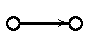
\includegraphics[width=0.34\textwidth]{figures/Fig_100_PDF185_Book173.pdf}
  \caption{练习 6.7 中的箭图 $Q$（原书 p.173）}
\end{figure}
\end{exercise}

\begin{exercise}\label{exer:quintic-all-orientations}
令 $W\colon\mathbb C\to\mathbb C$，$Z\mapsto\frac45Z^5+Z$，如例\ref{ex:quintic-thimbles}所述。对线性箭图 $L_4$ 的每一种箭头定向，求一组生成元，使其自同态环为该箭图的路径代数。
\end{exercise}

\begin{exercise}\label{exer:z2-zminus1-generators}
令 $W\colon\mathbb C^*\to\mathbb C$，$Z\mapsto Z^2+Z^{-1}$。求有向 Fukaya 范畴的一组生成元，并描述其自同态环。
\end{exercise}

\begin{exercise}\label{exer:two-sided-stops}
考察 $T^*S^1$，在一端放置 $k$ 个 stop，在另一端也放置 $k$ 个 stop。令 $L_{i,0}$ 是一条拉格朗日子流形，其一端从第一端第 $i$ 个与第 $i+1$ 个 stop 之间出发，另一端也止于第二端第 $i$ 个与第 $i+1$ 个 stop 之间；令 $L_{i,1}$ 从相同区间出发，但在另一端止于再往前一个区间（即第 $i+1$ 与第 $i+2$ 个 stop 之间）。
\begin{enumerate}[label=(\roman*)]
  \item 通过用这些曲线取锥来逼近任意曲线，证明它们生成 partially wrapped Fukaya 范畴。
  \item 计算这些拉格朗日子流形的自同态环。
  \item 现在考察 $W\colon\mathbb C^*\to\mathbb C$，$Z\mapsto Z^k+Z^{-k}$。解释这个 Lefschetz 纤维化的有向 Fukaya 范畴为何等价于本题中的 partially wrapped Fukaya 范畴。
\end{enumerate}
\end{exercise}

\chapterreview{%
\textbf{全章地位。}本章是同调镜像对称 A 侧的定义章。它先用开篇的 Morse 理论当练习场，让读者在有限维、可计算的设定里看清“复形—微分—分次”三件事，再把同一套机器搬到辛流形上，构造出基本 Fukaya 范畴，并依次给出 wrapped、partially wrapped、有向、相对、完整五种变体，最后讨论生成元。后文的曲面组合模型与所有 A 侧计算都以本章为入口。

\textbf{知识脉络。}Morse 复形由临界点张成，微分统计指数相差 $1$ 的流轨迹，$d^2=0$ 来自单参数轨迹族两端的符号相消；把 $M$ 换成余切丛的零截面、把梯度流换成 Hamilton 流，同一复形改由 $M$ 与 $\phi_\epsilon^hM$ 的交点张成，微分统计全纯二边形，Morse 指数随之变成交点的分次。若 Hamilton 函数只含动能项，交点便编码闭测地线，复形转而计算环路空间同调。把这一图景放到带柱状端的 Liouville 流形上：对象取正合紧致拉格朗日子流形，态射由横截交点张成，高阶积计数满足边界条件的伪全纯多边形；正合性保证面积由边界势差控制、求和有限，并排除泡，于是得到 $\mathbb Z_2$ 分次的 $A_\infty$ 预范畴，存在复体积形式时可提升为 $\mathbb Z$ 分次。变体一节再逐层放宽：允许浸入与局部系统；纳入非紧对象（wrapped，用 Reeb 弦与 $S_k$ 处理配对问题）；用 stop 截断 Reeb 流（partially wrapped，$U$-次数为零的态射，局部化）；用 Lefschetz 纤维化的 thimble 定义有向范畴；用除子与 Novikov 域处理紧致流形。

\textbf{核心结论。}（1）Morse 复形是上链复形，其上同调等于 $H^\bullet(M)$；在 $T^*M$ 中 $CF^\bullet(\phi_\epsilon^hM,M)$ 复现同一复形。（2）正合性使 Floer 乘积成为有限和：$\int_D\psi^*\omega=\sum_i\bigl(f_i(p_{i+1})-f_i(p_i)\bigr)$ 被紧致性控制；正合情形下两类泡都给出面积为零的映射，与 Gromov 紧致性矛盾，故 $\mu_k$ 满足 $A_\infty$ 关系。（3）$\mu_k$ 的次数为 $2-k$，交点次数为 $\deg x=(\Delta-(\theta_2-\theta_1))/\pi$；一般只有 $\mathbb Z_2$ 分次，Calabi--Yau 流形上可取 $\mathbb Z$ 分次。（4）包含链 $\mathrm{exFuk}^\bullet\subset\mathrm{wrFuk}^\bullet$；$\mathrm{wrFuk}^\bullet(T^*M)$ 由单个余切纤维生成，且 $D^\pi\mathrm{Fuk}^{\mathrm{wr}}T^*M\simeq D^\pi H^\bullet(\mathcal L_xM)$。（5）生成判据：若单位元 $1\in SH^\bullet(X)$ 落在开闭映射 $OC$ 的像中，则这组拉格朗日膜分裂生成 wrapped Fukaya 范畴。

\textbf{辨析与提醒。}其一，正合不是辛流形的一个技术条件，而是要求 $\theta$ 整体存在，因此正合辛流形必非紧致（否则 $\omega^n$ 是体积形式却上同调为零）；相对范畴与完整范畴正是为紧致流形补这个洞。其二，$\mathbb Z_2$ 与 $\mathbb Z$ 分次的差别不是记账问题：交点次数依赖 $\Omega$ 的相位沿路径的单值性，$\Omega=z^kdz$ 在 $k\ne-1$ 时甚至不给出底圆的分次，基本范畴为空。其三，wrapped 与普通 Fukaya 范畴的关系类似“有限生成模与有限维模”，partially wrapped 则是把某个子范畴的态射取逆的局部化；对象集逐层扩大，不能用同一套直觉混用。其四，定向与自旋结构、符号 $\sigma_\psi$ 是 $A_\infty$ 关系成立的实质条件，只有在 $\operatorname{char}k=2$ 时才可以暂时忽略。

\textbf{评注。}作者选择“Morse $\to$ Fukaya”的路线是有代价的：正文从未真正写下虚拟基本类或含时扰动的完整定义，模空间的光滑性、$S_k$ 的相干性、$k[[G]]$ 不是域时的极小模型，都只用“应当可以”“技术上相当复杂”带过。但这一取舍换来了全书最清晰的一条主线——读者始终知道每个定义是为解决哪个具体障碍而设：泡逼出正合性与带曲率结构，非紧对象逼出 wrapped，紧致流形逼出相对与完整范畴。真正该记住的不是定义本身，而是两个构造：拉格朗日手术即锥（$L_1+_xL_2\cong\operatorname{Cone}(x)$）与开闭映射检测生成。局限也要看清：曲面上用弧切分多边形得到的组合模型极其漂亮，却不能外推到高维，高维情形必须回到 Abouzaid 判据；而完整 Fukaya 范畴在本章只是框架，要做具体计算，仍应回到正合或相对设定。}
